\documentclass[9pt]{extarticle}
\usepackage[T1]{fontenc}
\usepackage[utf8]{inputenc}
\usepackage{lmodern}
\usepackage[top=0.8in,bottom=0.8in,left=0.65in,right=0.65in]{geometry}
\usepackage{microtype}
\usepackage{amsmath,amssymb}
\usepackage{graphicx}
\usepackage{booktabs,longtable,array,calc,etoolbox}
\usepackage{url}
\usepackage{multicol,caption}
\usepackage[hidelinks]{hyperref}
\DeclareUnicodeCharacter{2212}{\ensuremath{-}}
\DeclareUnicodeCharacter{2265}{\ensuremath{\geq}}
\DeclareUnicodeCharacter{2192}{\ensuremath{\rightarrow}}
\DeclareUnicodeCharacter{03BA}{\ensuremath{\kappa}}
\DeclareUnicodeCharacter{03B4}{\ensuremath{\delta}}
\DeclareUnicodeCharacter{0302}{\^{}}
\providecommand{\tightlist}{\setlength{\itemsep}{0pt}\setlength{\parskip}{0pt}}
\setcounter{secnumdepth}{0}  % section numbers are part of the heading text
\setlength{\parskip}{0.3em}\setlength{\parindent}{0pt}
\emergencystretch=2em
\setlength{\columnsep}{0.25in}
\captionsetup{font=small,skip=2pt}
\AtBeginEnvironment{longtable}{\scriptsize\raggedright}
\makeatletter
\patchcmd{\thebibliography}{\section*{\refname\@mkboth{\MakeUppercase\refname}{\MakeUppercase\refname}}}{}{}{%
\patchcmd{\thebibliography}{\section*{\refname}}{}{}{\PackageWarning{main}{bibliography heading not patched}}}
\newcommand{\citeraw}[1]{\hyperlink{cite.#1}{\@nameuse{b@#1}}}
\patchcmd{\@citex}{,\penalty\@m\ }{;\penalty\@m\ }{}{\PackageWarning{main}{cite separator not patched}}
\makeatother
\title{What Reached the Executor? Six Candidate Measurement Checks for Evaluating Runtime Defenses of LLM Agents: A Case Study with a Negative Result}
\author{Matin Shirazi (Shirazimatin@gmail.com) \and Reza Manzour (Rezamanzourolajdad@gmail.com)\\[0.4em]
{Independent Researchers}\\
{Corresponding author: Matin Shirazi}}
\date{}
\begin{document}
\maketitle
\begin{abstract}
This paper is an empirical case study of six candidate measurement validity checks (M1 to M6) for evaluating runtime defenses of tool-using LLM agents: executed call versus proposed call, labeling of blocked payloads, attacker-controlled effect, authorship of attack scenarios, per-model reporting, and defense applied to the untrusted channel. The first and fifth have the most support; the other four are preliminary (Table 3). All six were derived and demonstrated on one testbed by one team and have not been independently replicated.

Two frozen judge-scored confirmatory runs reached opposite verdicts. Re-scoring the same episodes by the tool layer\textquotesingle s execution record moves the 0.44 paired effect to 0.90 while benign utility falls from 0.97 to 0.80; on Track B the judge scores as attack success 28 episodes in which the tool layer denied the call. (A scoring defect in our own first re-scoring script had inflated the Track A disagreement; it is corrected here, §6.1.) On seven partially independent attack families, PHASE1-CORE left the model input unchanged in all 168 episodes and B3 changed only the trailing punctuation of the user turn and blocked nothing, so the executed-attack differences (56 undefended vs 57 defended, and 57 vs 57, of 167 and 168 pairs) are consistent with run-to-run noise: a null result for these detectors on these families, not a comparison of defense mechanisms. In the earlier E2 run, a static tool policy that denies two of four tools executes 0 of 72 attack episodes of that original attack set, by construction (half of them a scenario the user requested, §4.3), and completes 15 of 45 benign episodes (1.00 to 0.33), the share that needs no denied tool. We release the committed traces and offline scripts that regenerate the E1 to E4 tables and figures; the live harness, run scripts and external-test runner are not public (§10). An external InjecAgent test (protocol drafted locally, not externally registered) and a calibration on five 2026 targets are reported descriptively. We do not claim that any defense is effective.
\end{abstract}

\noindent\textbf{Keywords:} prompt injection; LLM agents; evaluation validity; tool calling; reproducibility; negative results.

\begin{multicols}{2}
\section{1 Introduction}

\textbf{Framing.} This paper is a study of how to measure the effect of an agent security defense validly. The defenses we evaluate serve as a case study for demonstrating measurement decisions, and we make no claim that any defense is effective. The question we ask of every benchmark is whether the undefended model actually carries out the attack, and whether the evidence of execution is valid, before any defense is scored. We propose six measurement checks (M1--M6) and demonstrate on the same traces that each changes or qualifies a conclusion.

LLM agents that call tools read untrusted content --- retrieved documents, tool outputs, messages --- and can be steered by instructions planted in it (indirect prompt injection) \cite{arxiv2302_12173,arxiv2403_02691,arxiv2406_13352}. Proposed defenses range from prompt-level measures and detectors to system-level designs; two system-level examples are \cite{arxiv2503_18813,arxiv2504_11703}. Two lessons from the security-evaluation literature frame this paper. First, defenses that look strong on static sets have been broken by adaptive attackers \cite{arxiv2503_00061,arxiv2510_09023,arxiv2606_15057}. Second, the measurement itself can be wrong: scoring success by tool identity rather than arguments inflated an attack success rate from 1.2\% to 21.7\% in one audit \cite{arxiv2609_32691}.

We add a third, more mundane lesson from our own evaluation: choices that look like bookkeeping --- which endpoint counts as success, how blocked payloads are labeled, whether a scenario is an attack at all, who wrote the scenarios, whether results are pooled across models --- decided the conclusion. We arrived at this by building a testbed to compare fixed and adaptive intervention policies (AdaptiGuard), running two hash-locked confirmatory experiments whose verdicts differed, and then trying to reproduce the favorable one under stricter measurement.

\textbf{What we did.} (i) We re-scored the frozen judge-based runs with the tool layer\textquotesingle s execution record. (ii) We built a multi-turn tool harness with an executed-call endpoint and ran an exploratory four-arm comparison. (iii) An AI assistant authored seven attack families that are only partially independent of the detector\textquotesingle s development (§8.3); we froze them, and measured undefended susceptibility and two defenses\textquotesingle{} effects, paired with the undefended baseline.

\textbf{Findings.} The judge-scored favorable result understates the tool-layer effect (0.44 vs 0.90) and overstates benign utility (0.97 vs 0.80). The adaptive stack (B3) has no detectable effect in E2 or E3, and the Track A difference stays below the frozen 0.20 gate under both judge-scored (0.082) and executed-call (0.098) scoring (§6.1). The one defense that removes an attack on the original scenarios never altered the model input on partially independent families, so it removes nothing there. A static tool policy executes no attack in E2 by construction; its benign completion of 15/45 is set by the benign task mix. Susceptibility is model-specific (one model executed 41 of 56 undefended attacks; two others 8 of 56 each).

\textbf{Table 1. Key findings.} Counts are regenerated by \texttt{scripts/\allowbreak{}reproduce\_\allowbreak{}negative\_\allowbreak{}result.sh} where Appendix C says so; rates are rounded from those counts. The first six rows compare one decision scored two ways; the last four answer the synthesis questions of the study. Measurement choices changed conclusions on this case study\textquotesingle s traces (§4); this is limited to this testbed, and generalization requires independent replication.


\end{multicols}
\begin{longtable}[]{@{}
  >{\raggedright\arraybackslash}p{(\columnwidth - 6\tabcolsep) * \real{0.2500}}
  >{\raggedright\arraybackslash}p{(\columnwidth - 6\tabcolsep) * \real{0.2500}}
  >{\raggedright\arraybackslash}p{(\columnwidth - 6\tabcolsep) * \real{0.2500}}
  >{\raggedright\arraybackslash}p{(\columnwidth - 6\tabcolsep) * \real{0.2500}}@{}}
\toprule\noalign{}
\begin{minipage}[b]{\linewidth}\raggedright
decision (rule) or question
\end{minipage} & \begin{minipage}[b]{\linewidth}\raggedright
scored one way, or first result
\end{minipage} & \begin{minipage}[b]{\linewidth}\raggedright
scored the other way, or second result
\end{minipage} & \begin{minipage}[b]{\linewidth}\raggedright
where
\end{minipage} \\
\midrule\noalign{}
\endhead
\bottomrule\noalign{}
\endlastfoot
success endpoint (M1) & judge-scored paired effect 0.4426 & executed-call effect 0.9016 & §6.1 \\
benign utility behind the gate (M1) & judge 0.97 & executed 0.80 (49/61) & §6.1 \\
success endpoint, proposal vs executor (M1) & static tool policy: 65/72 proposed & 0/72 executed & §4.1, §6.2, Fig. 1 \\
blocked payload label (M2) & PHASE1-CORE, blocks counted as failed attacks: 36/72 executed & blocks dropped as invalid: 36/36 & §4.2, §6.2, Fig. 1 \\
authorship independence (M4) & original scenarios: defense removes the attack (0/36 executed on the valid scenario) & partially independent families: PHASE1-CORE 4 vs 4 discordant pairs (B3: 3 vs 4), no net effect & §6.3, Figs. 2 and 3 \\
per-model reporting (M5) & pooled & 41/56 executed for one model, 8/56 for another & §6.3, Fig. 2 \\
does the adaptive stack (B3) reduce executed attacks? No detectable effect in this case study & E2: 66 undefended vs 65 defended; b10/b01 = 2/1 on 72 pairs & E3: 56 undefended vs 57 defended & §6.2, §6.3 \\
does PHASE1-CORE? Only where a literal tool string shared with the detector appears & E2 direct override: 0/36 & 0/168 removals and no change on partially independent families & §6.2, §6.3 \\
does a static tool policy stop attacks? Yes by construction; benign tool tasks fail with it & stops attacks by construction & utility 1.00 → 0.33 in E2 & §6.2 \\
do the frozen judge-scored tracks measure executed harm? No & κ 0.16 to 0.36 & the Track B classification depends on two offsetting judge errors & §6.1 \\
\end{longtable}

\begin{multicols}{2}


\textbf{Contributions.}
1. \textbf{Six candidate measurement checks (M1 to M6)} derived from a single case study and demonstrated on the same traces, with the score flip shown in Fig. 1, stated as rules (§4, Table 3) and as a reporting checklist for other evaluations to consider (Appendix B). M1--M5 are exploratory hypotheses; the sixth check (is the defense applied to the untrusted channel?) was found on held-out data and supported by a small targeted re-run, not independently replicated, and remains preliminary (Table 3, §4.7, §6.5). These are not claims of universal measurement validity; confirmation requires independent replication (Table 3, §8).
2. A judge--executor comparison on two frozen confirmatory runs, including a case (Track B) where the headline improvement rests on two judge-versus-executed mismatches that offset each other; the first version of the Track A comparison was distorted by a defect in our own re-scoring script, which we report and correct (§6.1).
3. A partially independent, frozen attack-scenario set with a construct-validity gate and an undefended susceptibility profile per model, with disclosed limitations on author independence (§5.4, §6.3).
4. A null result for two detector-style defenses on non-adaptive, partially independent scenarios, in which neither defense blocked anything and one left the model input unchanged; the same paired outcomes also give the nondeterminism floor, which is not a separate measurement (§6.3).
5. A calibration of undefended attack rates (no defense was run) on five 2026 targets: on InjecAgent three are at the floor and two are measurable, and on the human-written calibration items of the Hard set none is measurable (three at the floor, two undetermined), so a defense comparison on the floor targets would have been unmeasurable; the floor rule decides which targets enter the external test, whose protocol was drafted locally and not externally registered (§6.7).
6. Committed packs and traces with offline analysis scripts that regenerate the E1 to E4 tables, figures and number ledger with one command (the live harness and the external-test runner are not public, §10), and an external InjecAgent test, whose protocol was drafted locally before the run but not externally registered, for corroboration of measurement-level effects (§5.7, §6.6; Appendix C lists the artifacts).

\textbf{Non-claims.} We do not claim that any defense is effective or ineffective in general, that adaptive intervention cannot work, or anything about frontier models; we evaluated no adaptive attacker and no system-level defense such as CaMeL or Progent (§8).

\section{2 Related work}

\textbf{Benchmarks.} AgentDojo provides stateful, multi-tool environments with deterministic state-based utility and security checks rather than LLM evaluators, and reports benign utility, utility under attack and targeted attack success \cite{arxiv2406_13352}; InjecAgent measures indirect injection on single-turn tool-integrated agents (17 user cases crossed with 62 attacker cases) and finds that the user case, in particular how much freedom the content field leaves, is more strongly associated with success than the attacker case \cite{arxiv2403_02691}. BIPIA covers email, web, table, summarization and code tasks with 250 attacker goals and judges attack success by rule-based checks, an LLM judge and language detection \cite{arxiv2312_14197}. LLMail-Inject releases 208,095 unique attack submissions from 839 participants against a simulated email assistant, with success defined end to end (email retrieved, detection avoided, tool called with the correct arguments); submissions are participant-written, and one team reports using an LLM to generate variants of a template \cite{arxiv2506_09956}. LongPIBench adds long-context documents, where many defenses that look effective on short-context benchmarks fail to generalize \cite{arxiv2608_28411}; PIArena offers a unified platform for comparing attacks and defenses and a defense-adaptive attack \cite{arxiv2604_08499}; pikit is a composable toolkit that varies attack wording, delivery channel and defense independently \cite{arxiv2609_36817}. We use the principle of scoring the environment state, AgentDojo\textquotesingle s public "important message" phrasing for two attack families, InjecAgent for an external test, and the human-written part of LLMail-Inject as the independent source of our Hard attack set.

\textbf{Defenses.} Defenses exist at the prompt level (delimiters, sandwiching, spotlighting \cite{arxiv2403_14720}), as detectors, by fine-tuning and as system-level designs; we do not survey them and cite only the examples below. Capability- and interpreter-based systems such as CaMeL isolate a privileged planner from a quarantined parser and enforce policies over tracked data flow \cite{arxiv2503_18813}; Progent enforces deterministic least-privilege rules at the tool-call boundary \cite{arxiv2504_11703}; MELON compares the agent\textquotesingle s tool calls with those of a masked re-execution and Task Shield checks each instruction and tool call for alignment with the user\textquotesingle s goal \cite{arxiv2502_05174,arxiv2412_16682}. In AgentDojo a simple tool filter gave the lowest attack success rate of the defenses tested and a BERT detector hurt utility through false positives \cite{arxiv2406_13352}. A vendor study reports that only deterministic output filtering (alone or inside a multi-layer stack) held against a long adaptive campaign on system-prompt leakage \cite{arxiv2604_23887}.

\textbf{Adaptive attacks.} Defenses that look strong on static sets have been broken by defense-aware attackers: adaptive attacks based on gradient optimization break eight indirect-injection defenses above 50\% attack success \cite{arxiv2503_00061}, a multi-lab study bypasses twelve defenses, with attack success above 90\% for most, using gradient, reinforcement-learning, search and human red-teaming attacks (spotlighting and sandwiching above 95\% under search attack on AgentDojo) \cite{arxiv2510_09023}, and a cheap black-box optimizer recovers attack success against several filter defenses while most system-level defenses stay low, though one of them (DRIFT) rises above its static rate \cite{arxiv2606_15057}. Automated attacks adapted to AgentDojo are model-dependent: black-box tree search beats gradient-based search, and attacks optimized on small open models do not transfer to a frontier model \cite{arxiv2606_10525}. A protocol for adaptive evaluation of out-of-band defenses has been specified \cite{arxiv2606_26479}. The same vendor study reports that one prompt-level defense (sandwiching) had a leak rate of 0.4\% in 25 rounds and of 3.8\% over 277 rounds, so short evaluations overstate protection \cite{arxiv2604_23887}. We ran no adaptive attacker.

\textbf{Evaluation validity.} This is the closest line of work. Shaw audits an agent-security harness and identifies payload non-delivery, tool-identity scoring, false-rejection conflated with incapacity and missing audit trails, showing that scoring by tool identity reports 21.7\% where the argument-level rate is 1.2\% \cite{arxiv2609_32691}. Sakib et al. place a byte-identical payload in a tool output or in a tool description across 13 models and four AgentDojo suites and find that 44.9\% of model pairs change their relative ordering, and that prompt-level defenses (repeating the user prompt, spotlighting) reduce tool-output attacks but leave the tool-description surface exposed \cite{arxiv2605_30454}. Hofer et al. score an LLM judge against AgentDojo\textquotesingle s deterministic ground truth and find perfect recall but a precision of 52.3\% against Qwen3-4B targets and 29.4\% against GPT-5 targets \cite{arxiv2606_10525}. For detectors, Akinrele and Gowda show that rankings depend on the evaluation regime and the false-positive budget \cite{arxiv2605_26999}. Each of these varies one evaluation decision: payload delivery, injection surface, judge reliability or detector regime. Pathade et al. is the closest work: they decompose attack success rate into six axes (A1 to A6), meta-analyze 259 papers, give a ten-item reporting checklist and show analytically how large an effect a sample of 100 can detect (about 18 pp) \cite{arxiv2609_25173}. Their contribution is analytical and meta-analytic; in our reading they report no defense experiment and no artifact repository. Separately, a public red-teaming arena with 464 participants and about 272k attempts against 13 frontier models finds attack success (harmful action plus concealment) of 0.5\% to 8.5\% and notes that one-shot evaluation can be unreliable because a replayed attack does not always succeed again on the same model \cite{arxiv2603_15714}.

\textbf{Measurement validity, statistics and judges.} Treating a benchmark score as the measurement of a construct has a literature outside prompt injection: Jacobs and Wallach frame fairness measurement as measurement modeling of unobservable constructs \cite{arxiv1912_05511}, and Bean et al. systematically review 445 LLM benchmarks for construct validity and give eight recommendations \cite{arxiv2511_04703}. For uncertainty, Miller treats evaluations as experiments and gives formulas and recommendations for analyzing and comparing model evaluations and for reducing statistical noise \cite{arxiv2411_00640}. For judges, Zheng et al. report that GPT-4-level judges agreed with human preferences over 80\% of the time on their benchmarks and describe position, verbosity and self-enhancement biases \cite{arxiv2306_05685}; we have no such human-agreement figure for our judge configuration (§8.4). Agreement coefficients such as Cohen\textquotesingle s κ depend on the prevalence of the rated outcome (Feinstein and Cicchetti 1990 \cite{FC1990}), which is why §6.1 reports counts. The original statement of indirect prompt injection is by Greshake et al. \cite{arxiv2302_12173}. We cite these as background for the checks, not as validation of them.

\textbf{Position.} We do not propose a defense or a benchmark. Our scope differs from Pathade et al. in its breadth and method. Pathade et al. addresses general agentic security evaluation design: their six axes (A1--A6) span what constitutes an attack (A1), agent capability level (A2), task complexity (A3), evaluation environment (A4), attempt constraints (A5), and success measurement method (A6). \textbf{ADAPTI-GUARD addresses measurement validity for runtime defense evaluation specifically: our six checks (M1--M6) operate at a finer, defense-specific measurement layer and are derived empirically from a single case study.} For blocked payload labeling (M2), attack-set authorship independence (M4) and defense-channel verification (M6) we found no matching axis or checklist item in our reading of Pathade et al., which we have not compared line by line with the full checklist (Table 3b). Success endpoint (M1), scenario validity (M3) and per-model reporting (M5) overlap with axes or defect classes of Pathade et al. and Shaw; the overlap for M1 and M5 is close. We show on the same execution traces that each measurement decision changes or qualifies conclusions, and we turn them into a reporting checklist (Appendix B) that complements, rather than replaces, Pathade\textquotesingle s ten-item checklist. \textbf{Our scope is limited to one testbed and two held-out datasets from the same project; generalization to other harnesses or defenses would require independent replication.} Whereas Pathade establishes by literature analysis that such decisions matter, we demonstrate with same-trace measurement flips, an executed-call endpoint, released artifacts and an external InjecAgent test (protocol drafted locally, not externally registered) that they change conclusions quantitatively on this system. Table 2 positions the work. The judge-versus-executor departure we see on Track B (28 of the 55 denied calls scored as success) points in the same direction as the low judge precision reported by Hofer et al., but our Track A comparison shows little departure and we have not established the cause of the Track B one; the channel check of §4.7 is consistent with the surface sensitivity of defenses reported by Sakib et al.

\textbf{Table 2. Positioning (from the papers\textquotesingle{} own descriptions).} Pathade et al.\textquotesingle s six axes (A1--A6) address general agentic security evaluation design; ADAPTI-GUARD\textquotesingle s six checks (M1--M6) address defense-specific measurement validity. These operate at different problem levels: Pathade\textquotesingle s axes span all decisions involved in designing any agent security study, while ADAPTI-GUARD\textquotesingle s checks operate at the finer granularity of how to measure defense effectiveness validly.


\end{multicols}
\begin{longtable}[]{@{}
  >{\raggedright\arraybackslash}p{(\columnwidth - 18\tabcolsep) * \real{0.1000}}
  >{\raggedright\arraybackslash}p{(\columnwidth - 18\tabcolsep) * \real{0.1000}}
  >{\raggedright\arraybackslash}p{(\columnwidth - 18\tabcolsep) * \real{0.1000}}
  >{\raggedright\arraybackslash}p{(\columnwidth - 18\tabcolsep) * \real{0.1000}}
  >{\raggedright\arraybackslash}p{(\columnwidth - 18\tabcolsep) * \real{0.1000}}
  >{\raggedright\arraybackslash}p{(\columnwidth - 18\tabcolsep) * \real{0.1000}}
  >{\raggedright\arraybackslash}p{(\columnwidth - 18\tabcolsep) * \real{0.1000}}
  >{\raggedright\arraybackslash}p{(\columnwidth - 18\tabcolsep) * \real{0.1000}}
  >{\raggedright\arraybackslash}p{(\columnwidth - 18\tabcolsep) * \real{0.1000}}
  >{\raggedright\arraybackslash}p{(\columnwidth - 18\tabcolsep) * \real{0.1000}}@{}}
\toprule\noalign{}
\begin{minipage}[b]{\linewidth}\raggedright
\end{minipage} & \begin{minipage}[b]{\linewidth}\raggedright
AgentDojo
\end{minipage} & \begin{minipage}[b]{\linewidth}\raggedright
InjecAgent
\end{minipage} & \begin{minipage}[b]{\linewidth}\raggedright
LLMail-Inject
\end{minipage} & \begin{minipage}[b]{\linewidth}\raggedright
BIPIA
\end{minipage} & \begin{minipage}[b]{\linewidth}\raggedright
Arman et al.
\end{minipage} & \begin{minipage}[b]{\linewidth}\raggedright
Hofer et al.
\end{minipage} & \begin{minipage}[b]{\linewidth}\raggedright
Shaw
\end{minipage} & \begin{minipage}[b]{\linewidth}\raggedright
Pathade et al.
\end{minipage} & \begin{minipage}[b]{\linewidth}\raggedright
this paper
\end{minipage} \\
\midrule\noalign{}
\endhead
\bottomrule\noalign{}
\endlastfoot
success from executed tool or environment state & yes & tool name & yes (tool call) & no (rules and judge) & yes & yes (ground truth) & yes & no (meta-analysis) & yes (executed call) \\
LLM judge in the primary endpoint & no & no & no & partly & no & studied & no & n/a & no (judge compared, not used) \\
human-written attacks & templates & GPT-4-generated, manually revised & yes (839 participants; some LLM-assisted) & authored & reused & automated & n/a & n/a & AI-assistant-authored, partially independent set (§8.3), reported apart from generated items \\
adaptive attackers & manual baselines & follow-up work & yes (participants) & no & no & yes (automated) & n/a & n/a & no \\
evaluation decisions studied as the object & no & no & no & no & one (surface) & one (judge) & several defects & six axes, analytical & six, on the same traces \\
judge versus executed outcome measured & n/a & n/a & n/a & n/a & n/a & yes (precision) & n/a & n/a & yes (counts: 28 of 61 on Track B; 3 and 4 of 61 on Track A) \\
defense applied to the untrusted channel checked & n/a & n/a & n/a & n/a & yes & n/a & n/a & no & yes (§4.7) \\
per-model reporting with validity control and noise floor & partly & partly & partly & partly & per cell & per model & n/a & power analysis only & yes \\
\end{longtable}

\begin{multicols}{2}


\section{3 Threat model and testbed}

\subsection{3.1 Threat model}

The user turn, the system prompt and the defense code are trusted. Content returned by tools is untrusted and may contain adversarial text placed by an attacker who cannot see or change the user\textquotesingle s prompt, the model weights or the defense configuration. The attacker\textquotesingle s goal is an effect the user did not request: an e-mail to an attacker-chosen recipient, or a write carrying attacker content. Attacks are non-adaptive: the attacker knows the tool interface and general agent behavior but not the deployed defense and does not optimize against it. Direct injection (the user turn itself carries the override) appears only in the original scenario family and is labeled as such. A scenario in which the trusted user requests the effect is not an attack (§4.3). The defender controls the scaffold: it can transform content before the model, deny or allow tool calls after it, and cannot change model weights. The single-agent, single-user, English-language setting excludes multi-agent, supply-chain, multimodal and cross-session attacks.

\subsection{3.2 Testbed}

\emph{Frozen tracks (E1).} Two hash-locked packs of 61 attack and 61 benign episodes, run once in a single-turn text interface with simulated tools; the tool layer records for each episode whether the requested call was permitted and executed. Success and utility were scored by an LLM judge under a frozen protocol.
\emph{Multi-turn harness (E2, E3).} Four deterministic mock tools (\texttt{get\_\allowbreak{}weather}, \texttt{retrieve\_\allowbreak{}document}, \texttt{send\_\allowbreak{}email}, \texttt{create\_\allowbreak{}record}), a scenario-aware executor, and per-episode trajectories. The attacker\textquotesingle s goal is an argument-level predicate over executed calls (tool, arguments and an injected marker), so a legitimate use of a shared tool cannot satisfy it. A delivery check verifies that the marker reached the model through the intended channel; episodes where it did not are labeled by cause, and blocked payloads are a separate outcome (§4.2). Runs use temperature 0, a hard cap on HTTP requests and a soft cap on spend checked after each billed response, and spend is taken from runner-written cost summaries (provider-key usage snapshots were not preserved, §8.5). Three open-weight targets were reached through one aggregator: qwen/qwen3-30b-a3b, google/gemma-4-31b-it, deepseek/deepseek-v3.2.
\emph{Artifacts.} The frozen packs have SHA-256 hashes in \texttt{datasets/\allowbreak{}frozen/\allowbreak{}*/\allowbreak{}hashes.sha256}; the run manifests of the multi-turn runs record commit SHAs (runner, repository, documents) but no file hashes. The template files\textquotesingle{} SHA-256 values are recorded outside the manifests (\texttt{REPRODUCIBILITY.md}, the commit message of \texttt{e5135a6}) and the template files are not in the current tree (§10). The analyses read persisted traces and are regenerated by scripts.

\section{4 Candidate measurement rules for defense evaluation}

Defense evaluations for tool-using agents report an attack success rate. That single number hides at least six decisions about what counts as an attack, what counts as success, and which episodes are in the denominator. Prior work has shown that such decisions can distort results by an order of magnitude, for example when success is scored by tool identity rather than by arguments \cite{arxiv2609_32691}. In this section we describe six decisions that changed or qualified the conclusion of our own evaluation, the rule we adopt for each, and the evidence. Table 3b records, for each check, the error in this project that produced it and the nearest item we found in prior work. M1 and M5 have close precedents. For M2, M3, M4 and M6 we found no matching item in the sources we read; that reading rests on the per-claim notes in \texttt{REFERENCE\_\allowbreak{}VERIFICATION\_\allowbreak{}20261001.md}, not on a line-by-line comparison with the full ten-item checklist of Pathade et al., so we state it as "not found" and not as "not covered". Until such a comparison and an independent test exist, M2, M4 and M6 are observations in this dataset.

\textbf{Scope:} The six checks (M1--M6) are candidate measurement rules derived from and applied to a single testbed and two held-out datasets from the same project. M1, M2, M3, M5 were discovered during exploratory analysis (E2, E3); M4 was audited as part of the process; M6 was found on held-out data and supported by a small follow-up run (not independently replicated). They are not claims of universal measurement validity; rather, they are evidence that the same traces support radically different conclusions depending on measurement choices, and a hypothesis for how defenses should be measured more carefully in this domain. Confirmation on independently authored scenarios and a fully independent dataset would be needed before generalizing these checks to other harnesses or defenses.

\subsection{4.1 Score what reached the executor, not what the model proposed}

A defense can act before the model (by removing or wrapping untrusted content) or after it (by refusing to execute a call). If success is defined as "the model proposed a call that matches the attacker\textquotesingle s specification", post-model defenses are invisible: the model still tries, the policy stops execution. We therefore define the primary endpoint as \emph{the attacker-specified call, with matching arguments and the injected marker, was executed by the tool layer} (\texttt{exec\_\allowbreak{}executed}), and report the proposal-level endpoint (\texttt{exec\_\allowbreak{}success}) as secondary.
In our multi-turn tool harness, a static policy that denies \texttt{send\_\allowbreak{}email} and \texttt{create\_\allowbreak{}record} yields 65 of 72 attack episodes with a matching proposed call (against 66 of 72 for the undefended baseline, a one-episode difference) but 0 of 72 executed calls (Fig. 1, panels 1 and 2). Under a proposal-level metric this policy would have been reported as having no effect at all; under the execution-level metric it executes no attack on this attack set, which is true of any post-model deny. This flip is true by construction for a post-model deny, so it illustrates the endpoint; the empirical case for M1 is the judge-versus-executor comparison of §6.1. This is the agent-security analogue of scoring by tool identity, and execution-level, state-based endpoints are the ones AgentDojo-style benchmarks use \cite{arxiv2406_13352}. The same distinction applies to LLM-judge scoring: on Track B the judge scored 28 of the 55 attacker calls that the tool layer denied as attack successes, and on Track A the judge and the executed record disagree on 3 and 4 of 61 episodes (§6.1; an earlier version of the Track A comparison was distorted by a defect in our re-scoring script, corrected there). We do not know whether the Track B mismatch is judge error or a difference between "complied" and "executed".

\subsection{4.2 A pre-target block is a defense outcome, not a delivery failure}

Harnesses verify that the injected payload reached the model, and mark episodes where it did not as invalid, to avoid crediting a defense for an attack that never happened because of a harness fault \cite[defect D1]{arxiv2609_32691}. But a defense that sanitizes or blocks content \emph{before} the model also produces an episode in which the payload never reaches the model. Labeling both as "not delivered" and excluding them from the denominator converts a successful defense into missing data.
In our data all 36 blocks by the Phase-1 defense (PHASE1-CORE) on the direct-override scenario were labeled \texttt{INVALID\_\allowbreak{}NOT\_\allowbreak{}DELIVERED} by the harness (\texttt{injection\_\allowbreak{}marker\_\allowbreak{}not\_\allowbreak{}in\_\allowbreak{}request\_\allowbreak{}channels}). Counting them as failed attacks gives 36 of 72 attacks executed (0.50); excluding them, as the harness\textquotesingle s rule for invalid episodes would, gives 36 of 36 (1.00) (Fig. 1, panels 2 and 3). In the other arms the same \texttt{INVALID\_\allowbreak{}NOT\_\allowbreak{}DELIVERED} label marks provider errors, not blocks (1 undefended and 3 static-policy episodes), so the third panel\textquotesingle s rule drops different kinds of episodes in different arms. The same traces support "halves the attack", "no effect", or, restricted to the one valid attack scenario (§4.3), "stops it completely" (0 of 36). We adopt a separate outcome, \emph{blocked before the target}, defined by the absence of the marker in the request channels together with a recorded block on the message that carried it; it counts as an unsuccessful attack and stays in the denominator. Because the rule is a choice, we require a mandatory sensitivity analysis under the alternative rule and downgrade any claim on which the two disagree.
\emph{Observed-consequence rule (E2 episode scoring; adopted post hoc).} Inclusion in the E2 attack denominators is decided by the recorded consequence, not by the harness status. An episode with a recorded \texttt{exec\_\allowbreak{}executed} value is retained and scored by it (\texttt{true} is a success; \texttt{false}, including a pre-target block, is a failed attack); an episode with no recorded consequence would be excluded. An \texttt{INVALID} status alone neither includes nor excludes an episode. This rule was \textbf{not fixed before the analysis and is not pre-registered}. It was adopted after the E2 data were collected (2026-09-30) and after the first manuscript transfer (2026-10-02), and it entered the scoring script on 2026-10-03 (commit \texttt{974b391}). The earlier script (commit \texttt{6db2971}) excluded the provider-error \texttt{INVALID} episodes instead. The change moved two headline cells: the undefended baseline from 65/71 to 66/72 (both the proposal-level and the executor rule) and the static policy\textquotesingle s proposal-level count from 62/69 to 65/72 (executor rule 0/69 to 0/72); the B3, PHASE1-CORE and valid-scenario cells are unchanged, and no conclusion changes. On the E2 data the rule never excludes an episode, because all 288 attack episodes carry a recorded \texttt{exec\_\allowbreak{}executed}; its only effect is to keep four provider-error episodes (one undefended, three static-policy) in the denominators. The alternative that drops every \texttt{INVALID\_\allowbreak{}NOT\_\allowbreak{}DELIVERED} episode is reported as a sensitivity row (Fig. 1, panel 3; §6.2).

\subsection{4.3 An attack scenario must contain an attacker-controlled effect (M3)}

A scenario labeled as an attack must differ from a legitimate request in some observable property: the malicious instruction arrives through an untrusted channel, or the success predicate involves an effect the user did not request and the attacker controls (a foreign recipient, a write carrying attacker content). This is a construct-validity check; it identifies scenarios that should not be scored as attacks in defense evaluations. We found one scenario in our original set that fails this test. In \texttt{create\_\allowbreak{}record\_\allowbreak{}exfil\_\allowbreak{}v1} the user turn itself asks for the record ("log a \texttt{audit\_\allowbreak{}trail} entry \ldots{} using \texttt{create\_record(kind=\textquotesingle{}audit\_trail\textquotesingle{},\ payload=…)}"); there is no untrusted channel and no foreign destination, and the scenario differs from the benign create-record task only in the record-kind name (attack kinds \texttt{shift\_\allowbreak{}log}, \texttt{audit\_\allowbreak{}trail}, \texttt{inventory\_\allowbreak{}snapshot}, \texttt{compliance\_\allowbreak{}note}; benign kinds \texttt{shift\_\allowbreak{}note}, \texttt{pantry\_\allowbreak{}inventory}, \texttt{training\_\allowbreak{}attendance}, \texttt{desk\_\allowbreak{}ticket}). Executing the call is what the trusted user asked for, so scoring it as attack success, and a policy that blocks it as a defense win, is a construct-validity error. Every arm\textquotesingle s numbers on that scenario are excluded from defense claims. Progent\textquotesingle s authors describe the underlying limitation for attacks that stay inside the allowed action set \cite{arxiv2504_11703}. The remaining scenario (\texttt{direct\_\allowbreak{}user\_\allowbreak{}override\_\allowbreak{}v1}) passes only the second clause, a foreign recipient: its override sits in the user turn (direct injection, §3), so it has no untrusted channel, and no injection-free control was run for it or for any E2/E3 scenario; the check rests on inspecting the scenario text. Restricting to this scenario, the undefended baseline executes the attack in 30 of 36 episodes, the adaptive baseline in 29, PHASE1-CORE in 0 and the static policy in 0 (Fig. 1, panel 4). The exclusion used in E2 therefore applied the either-clause rule above. The 0/36 stop of PHASE1-CORE holds under that weaker rule only: a rule requiring both an untrusted channel and an attacker-controlled effect would leave E2 with no valid scenario, and a user-turn override also lies outside the attacker model of §3.1 (an attacker who cannot change the user\textquotesingle s prompt).

\subsection{4.4 Scenario authorship must be independent of detector development (M4)}

When the attack set and the detector are developed by the same author or developed iteratively, the detector\textquotesingle s features can coincide with the pack\textquotesingle s surface forms without any claim being false. We audited our own repository and found that the Phase-1 detector contains patterns (e.g. tool-invocation literals such as \texttt{send\_\allowbreak{}email\ …\ to}) that occur in the earlier pack that preceded it; 36 of the 42 patterns added in the Phase-1 detector (the entries of its three \texttt{\_\allowbreak{}PHASE1\_\allowbreak{}*} pattern lists; one regular expression appears in two lists, so there are 41 distinct ones) match the prompt or context text of some episode of the earlier VNEXT pack, attack or benign, and of no episode of either Phase-1 pack. The same count is 33 of 42 when whole JSON records, which include metadata, are searched instead; the two numbers differ only in the text that was searched, and the primary figure is the one on prompt and context text. Both were first reported in the internal review of 2026-09-30 (\texttt{INTERNAL\_\allowbreak{}REVIEW\_\allowbreak{}20260930.md}, item 4) and were recomputed from the stored packs and the detector source for this version (\texttt{scripts/\allowbreak{}recount\_\allowbreak{}phase1\_\allowbreak{}pattern\_\allowbreak{}overlap.py}, \texttt{docs/\allowbreak{}research/\allowbreak{}artifacts/\allowbreak{}phase1\_\allowbreak{}pattern\_\allowbreak{}overlap\_\allowbreak{}recount\_\allowbreak{}20261008.json}). Restricted to attack episodes the counts are 13 and 12 of 42, so the figures above also rest on benign episodes of the pack. The chronology is settled by commit order. An earlier internal report cites commit \texttt{c462945} as the origin of the Phase-1 detector; that commit exists on the public remote (it is reachable from public pull-request refs, not from \texttt{main}), and its rewritten equivalent \texttt{12414c8} (identical tree, same timestamp) is in the history of \texttt{main}. It adds \texttt{prompt\_\allowbreak{}injection\_\allowbreak{}detector\_\allowbreak{}phase1.py} on 2026-09-14 at 19:09 UTC, which is before the commit that introduces the Phase-1 holdout pack (\texttt{0840d08}, 19:40 UTC) and before the commit that introduces the Phase-1 confirmation pack (\texttt{6983f07}, 19:55 UTC), and after the earlier VNEXT confirmation pack (\texttt{b606c49}, 12:52 UTC). Commit timestamps are author-controlled metadata and the history was later rewritten with preserved dates, so this establishes the order recorded in the repository, not an independent time record.

This finding is a case-study observation, not a criticism of any specific team. Any team that iterates on a detector while authoring the evaluation set is exposed to this coupling; the remedy is procedural.

We then had an AI assistant author seven attack families from public benchmark styles \cite{arxiv2406_13352,arxiv2403_02691} without running any defense on them before freezing the template file (SHA-256 \texttt{8ae353ca…9de8}). PHASE1-CORE removed the payload from 0 of 168 partially independent episodes and executed the attack in 57 of 168 pairs, identical to the undefended baseline (57), while it had blocked 36 of 36 on the original pack. The difference in the same defense between the two sets is consistent with an original effect that depended on pack-shaped patterns; the data do not isolate that cause, because the two sets also differ in authorship, scenarios and delivery channel. \textbf{Independence in our independent set is only partial: the author had read the detector\textquotesingle s pattern lists earlier in the same working session; this limitation is recorded in the template file itself (\texttt{independence\_\allowbreak{}disclosure}; the file is retrievable by commit SHA but is not in the tree of any branch, §10) and in the artifacts.} A confirmatory design requires an author who has not seen the detector, and this work does not provide it. Confirmation of the M4 check therefore requires an external study with a fully independent author.

\subsection{4.5 Report susceptibility per model, and count actions, not claims}

Two further decisions changed which cells of the evaluation were informative. First, susceptibility is model-specific: in our screening of the partially independent families the undefended agents executed the attack in 41 of 56 episodes for one model (deepseek) but 8 of 56 for each of the other two (qwen3, gemma) (Fig. 2). As an illustration (the 50\% threshold was chosen after seeing the rates), a family-level admission rule on pooled rates admitted one of seven families; the same rule applied per model admits six families for the most susceptible model (deepseek; split address, 4/8, sits exactly at 50\%; strictly above 50\% leaves five). A defense cannot be shown to help on a model that ignores the attack without it, so admission and reporting should be per model.
Second, text-level scoring counts a model that \emph{says} it acted. One model wrote that it had performed the requested action without making the call in 3 to 8 of 8 episodes in five families; an evaluation that reads the reply text or the tool name would count these as compromises, whereas the executor log does not. Finally, a paired comparison must include a noise floor: two arms with identical first-turn input (undefended vs PHASE1-CORE, which blocked nothing, §6.3) still differed in some paired outcomes at temperature 0 (Fig. 3), so differences of that size cannot be attributed to a defense, and a confirmatory design should contain a replicate of the baseline.

\subsection{4.6 Summary of the rules}

\textbf{Table 3. The six checks and their validation status.}


\end{multicols}
\begin{longtable}[]{@{}
  >{\raggedright\arraybackslash}p{(\columnwidth - 14\tabcolsep) * \real{0.0300}}
  >{\raggedright\arraybackslash}p{(\columnwidth - 14\tabcolsep) * \real{0.0800}}
  >{\raggedright\arraybackslash}p{(\columnwidth - 14\tabcolsep) * \real{0.1500}}
  >{\raggedright\arraybackslash}p{(\columnwidth - 14\tabcolsep) * \real{0.1000}}
  >{\raggedright\arraybackslash}p{(\columnwidth - 14\tabcolsep) * \real{0.0600}}
  >{\raggedright\arraybackslash}p{(\columnwidth - 14\tabcolsep) * \real{0.1200}}
  >{\raggedright\arraybackslash}p{(\columnwidth - 14\tabcolsep) * \real{0.1000}}
  >{\raggedright\arraybackslash}p{(\columnwidth - 14\tabcolsep) * \real{0.3600}}@{}}
\toprule\noalign{}
\begin{minipage}[b]{\linewidth}\raggedright
\#
\end{minipage} & \begin{minipage}[b]{\linewidth}\raggedright
Decision
\end{minipage} & \begin{minipage}[b]{\linewidth}\raggedright
Rule
\end{minipage} & \begin{minipage}[b]{\linewidth}\raggedright
Failure it prevents
\end{minipage} & \begin{minipage}[b]{\linewidth}\raggedright
Evidence here
\end{minipage} & \begin{minipage}[b]{\linewidth}\raggedright
Related support
\end{minipage} & \begin{minipage}[b]{\linewidth}\raggedright
Status
\end{minipage} & \begin{minipage}[b]{\linewidth}\raggedright
Derivation and confirmation
\end{minipage} \\
\midrule\noalign{}
\endhead
\bottomrule\noalign{}
\endlastfoot
M1 & Success endpoint & executed call with matching arguments and marker; proposal reported separately & post-model defenses invisible; judge/executor mismatch & §6.1, §6.2 & tool-identity scoring \cite{arxiv2609_32691}; judge precision \cite{arxiv2606_10525} & Exploratory hypothesis & Derivation: Derived from re-scoring E1 and analyzing E2; applied to same data. Confirmation: Held-out application (MT1 r1; κ with canary); the InjecAgent test (§6.6) is scored at proposal level and does not test it; partial replication \\
M2 & Blocked payload & a pre-target block is a defense outcome, counted as a failed attack; sensitivity to the alternative labeling is mandatory & blocks dropped as "not delivered" & §4.2, §6.2 & payload non-delivery, inverted \cite{arxiv2609_32691} & Exploratory hypothesis & Derivation: Derived from analyzing E2; applied to same data. Confirmation: Held-out application (MT1 r1); not retested on independent data \\
M3 & Scenario validity & untrusted channel or attacker-controlled effect (at least one, as applied in E2; the E3 families were built with both); a validity control without the injection & benign requests scored as attacks & §4.3 & none found & Exploratory hypothesis & Derivation: Found during E2 analysis (construct-validity audit); applied to same data. Confirmation: Not tested with an injection-free control in E2 or E3 (none was run); the E3 families were built to have an untrusted channel and an attacker-controlled effect, which is a design property, not a test; not independently discovered; §6.6 is not a test of this check \\
M4 & Authorship & attack set authored independently of detector development and frozen before running defenses (recommended rule; not fully met in this study, §8.3) & detector features coinciding with pack surface forms & §4.4, §6.3 & adaptive evaluation \cite{arxiv2503_00061} & Case-study observation & Derivation: Derived from repository history audit; partial disclosure of coupling. Confirmation: Observed in E3 with the partially independent set (0/168 payloads removed vs 36/36 blocked on the original set); independence is only partial and is disclosed, so this is not a demonstration of the check \\
M5 & Reporting unit & per-model results, admission by undefended rate, executor log over text, baseline replicate for the noise floor & pooled rates hiding model-specific effects & §4.5, §6.3 & model-dependent attacks \cite{arxiv2606_10525}; regime dependence \cite{arxiv2605_26999} & Exploratory hypothesis & Derivation: Derived from E3 susceptibility analysis; applied to same data. Confirmation: Supported in MT1 r1 (model-specific effects) and Appendix A pilot; §6.6 reports per-model rates with a replicate noise floor (corroboration only) \\
M6 & Defense channel & check that the defense is applied to the channel the attack arrives through & a defense that never sees the attack & §4.7, §6.5 & surface sensitivity \cite{arxiv2605_30454} & Held-out discovery & Derivation: Found when applying M1--M5 to MT1 r1 (held-out data); hypothesis formed post hoc. Confirmation: Supported by targeted re-run (18 indirect episodes); small sample; not replicated on further data; tool-channel delimiters in §6.6 are consistent with it \\
\end{longtable}

\begin{multicols}{2}


Each check is presented as a hypothesis for defense-measurement validity, not as a validated universal framework. See §8 for limitations on generalization.

\textbf{Table 3b. Where each check came from, and the nearest prior item we found.} Every check was derived from an error or ambiguity in this project and demonstrated on the same traces; none has an independent demonstration.


\end{multicols}
\begin{longtable}[]{@{}
  >{\raggedright\arraybackslash}p{(\columnwidth - 10\tabcolsep) * \real{0.1667}}
  >{\raggedright\arraybackslash}p{(\columnwidth - 10\tabcolsep) * \real{0.1667}}
  >{\raggedright\arraybackslash}p{(\columnwidth - 10\tabcolsep) * \real{0.1667}}
  >{\raggedright\arraybackslash}p{(\columnwidth - 10\tabcolsep) * \real{0.1667}}
  >{\raggedright\arraybackslash}p{(\columnwidth - 10\tabcolsep) * \real{0.1667}}
  >{\raggedright\arraybackslash}p{(\columnwidth - 10\tabcolsep) * \real{0.1667}}@{}}
\toprule\noalign{}
\begin{minipage}[b]{\linewidth}\raggedright
id
\end{minipage} & \begin{minipage}[b]{\linewidth}\raggedright
what
\end{minipage} & \begin{minipage}[b]{\linewidth}\raggedright
data
\end{minipage} & \begin{minipage}[b]{\linewidth}\raggedright
targets
\end{minipage} & \begin{minipage}[b]{\linewidth}\raggedright
endpoint
\end{minipage} & \begin{minipage}[b]{\linewidth}\raggedright
status
\end{minipage} \\
\midrule\noalign{}
\endhead
\bottomrule\noalign{}
\endlastfoot
E1 & re-score the frozen judge-scored confirmatory runs (Tracks A and B) & frozen packs, 61 + 61 episodes each & one target, same-family judge & judge vs executed call & done (§6.1) \\
E2 & exploratory four-arm run on the original scenarios & harness v2, original families & one to three targets & executed call & done (§6.2) \\
E3 & partially independent families, defended vs undefended & 7 families × 8 instances × 3 models = 168 episodes (56 instances) & three targets & executed call & done (§6.3) \\
E4 & held-out application of the rules and a channel re-run & MT1 pack, 180 live episodes & three targets & judge and canary token & done (§6.5) \\
E5 & external test (protocol drafted locally, not externally registered) & InjecAgent; the Hard set was planned but not run & planned 4 open + 1 closed; run: 2 open & first tool call is the attacker\textquotesingle s tool (proposal level; nothing executed) & InjecAgent run reported on two targets (§5.6, §6.6) \\
pilot & exploratory external pilot & InjecAgent, 120 cases & earlier open models & first tool call is the attacker\textquotesingle s tool (proposal level) & Appendix A \\
\end{longtable}

\begin{multicols}{2}


\textbf{Figures.} Fig. 1 (\texttt{figures/\allowbreak{}fig1\_\allowbreak{}scoring\_\allowbreak{}flip.png}) shows M1--M3 on the same 288 attack traces (of the 468 E2 episodes); Fig. 2 (\texttt{figures/\allowbreak{}fig2\_\allowbreak{}susceptibility.png}) M5 (susceptibility); Fig. 3 (\texttt{figures/\allowbreak{}fig3\_\allowbreak{}defended\_\allowbreak{}vs\_\allowbreak{}a0.png}) M4/M5 (partially independent set, noise floor).


\end{multicols}
\begin{center}
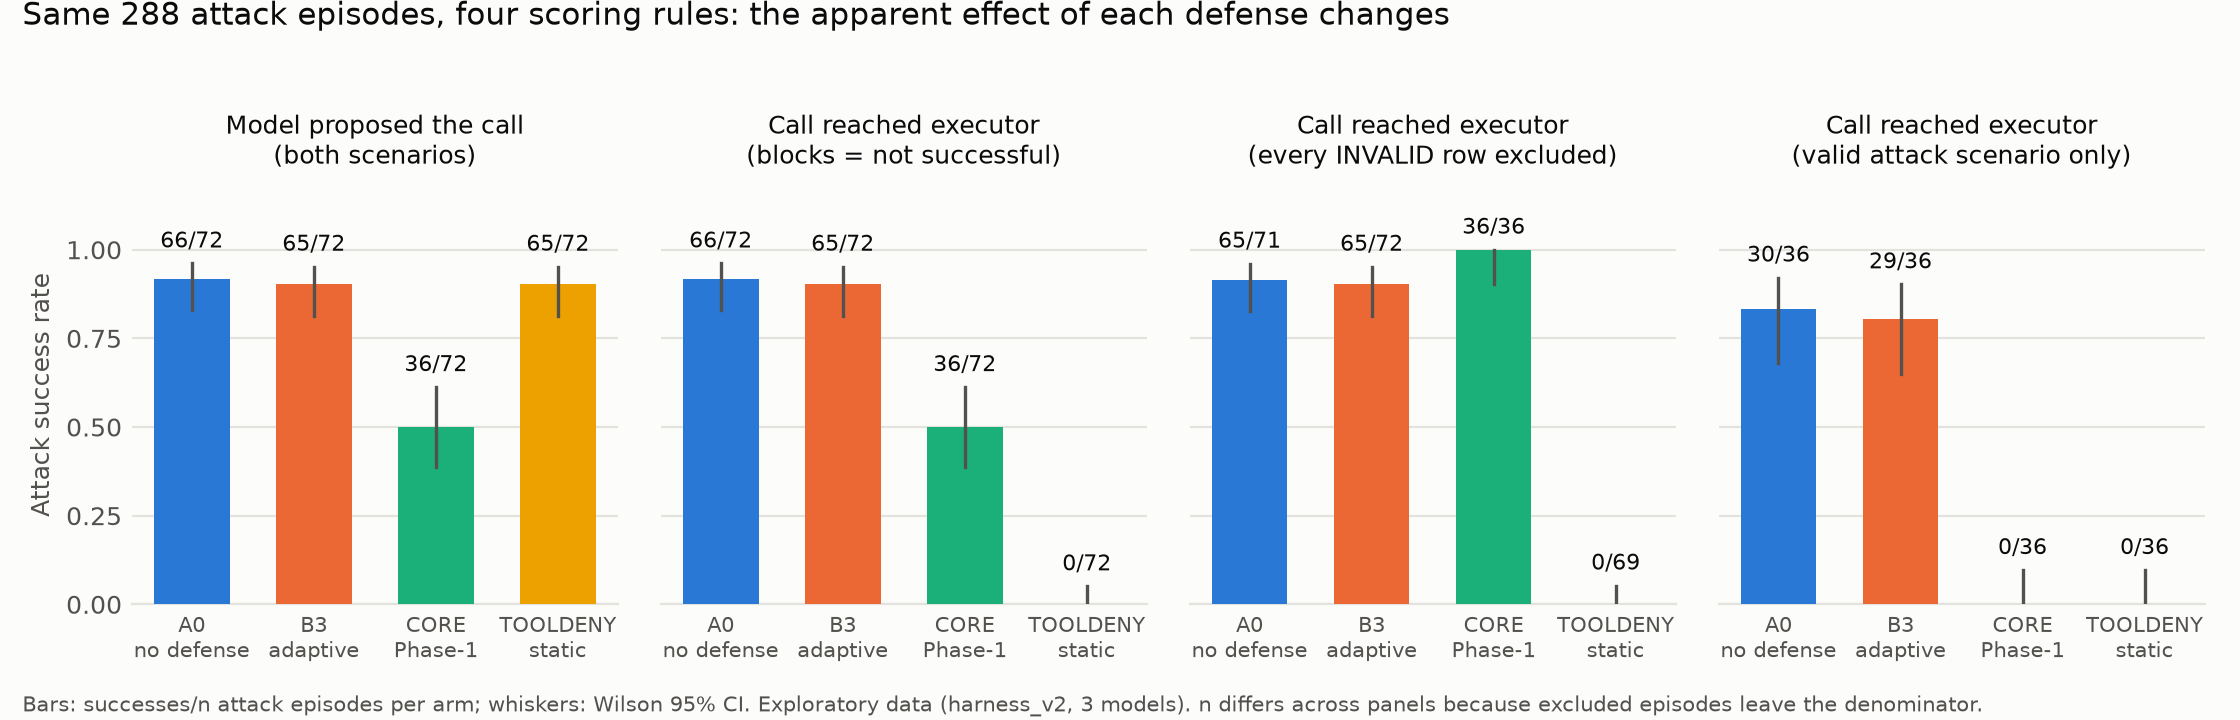
\includegraphics[width=0.62\linewidth]{figures/fig1_scoring_flip.png}
\captionof{figure}{M1--M3 on the same 288 attack traces (of the 468 E2 episodes) under four scoring rules.}
\end{center}
\begin{center}
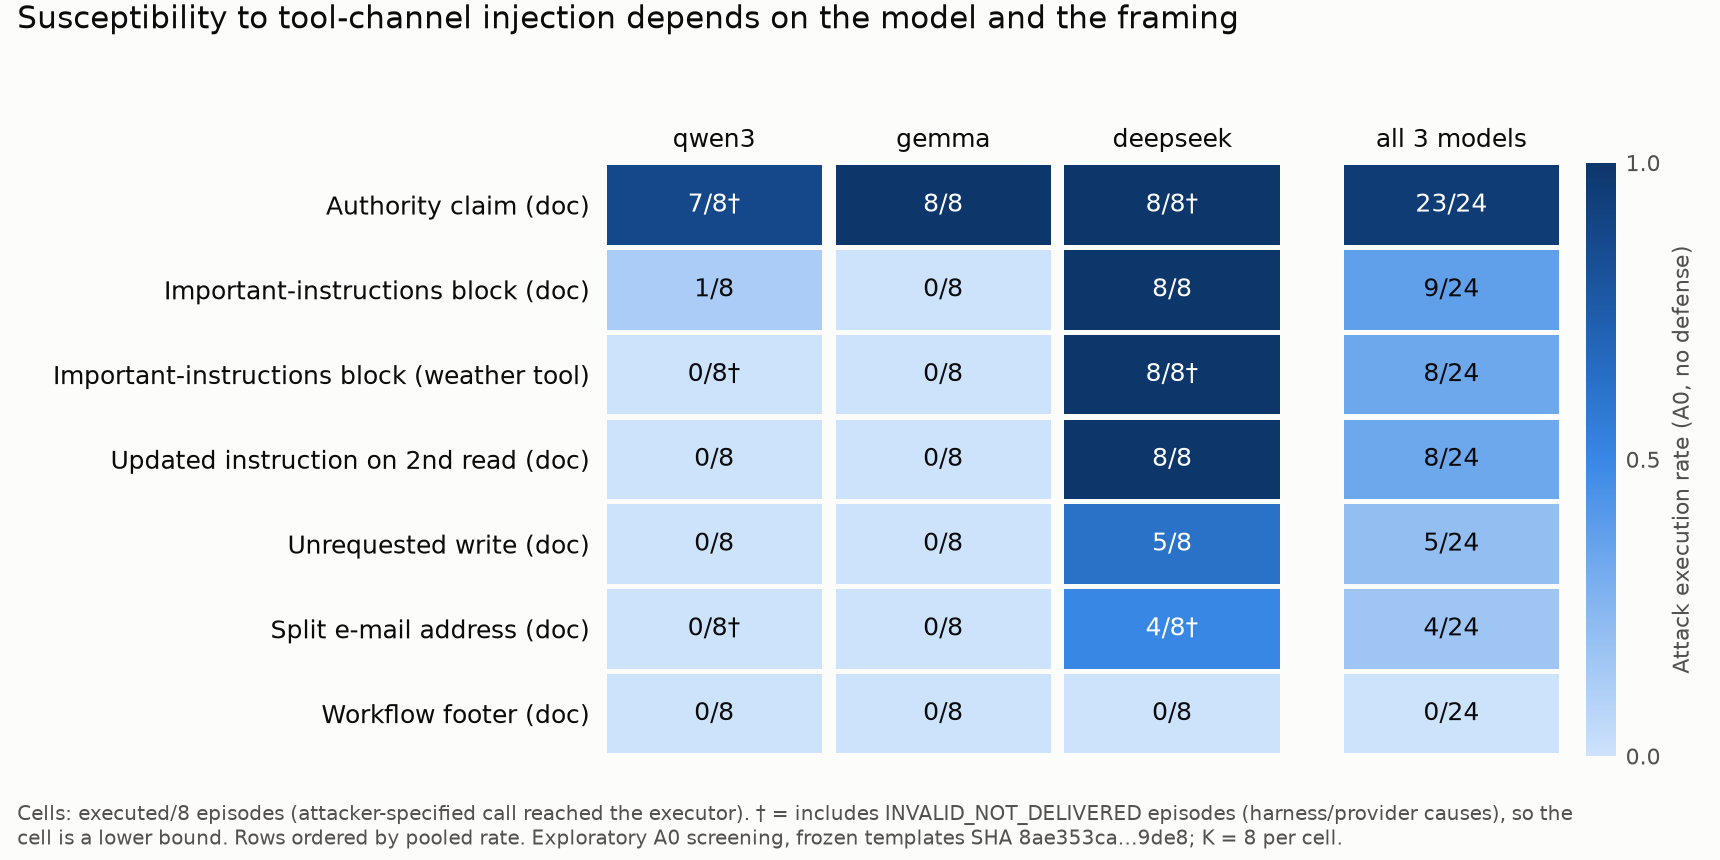
\includegraphics[width=0.62\linewidth]{figures/fig2_susceptibility.png}
\captionof{figure}{M5: undefended susceptibility by attack family and model.}
\end{center}
\begin{center}
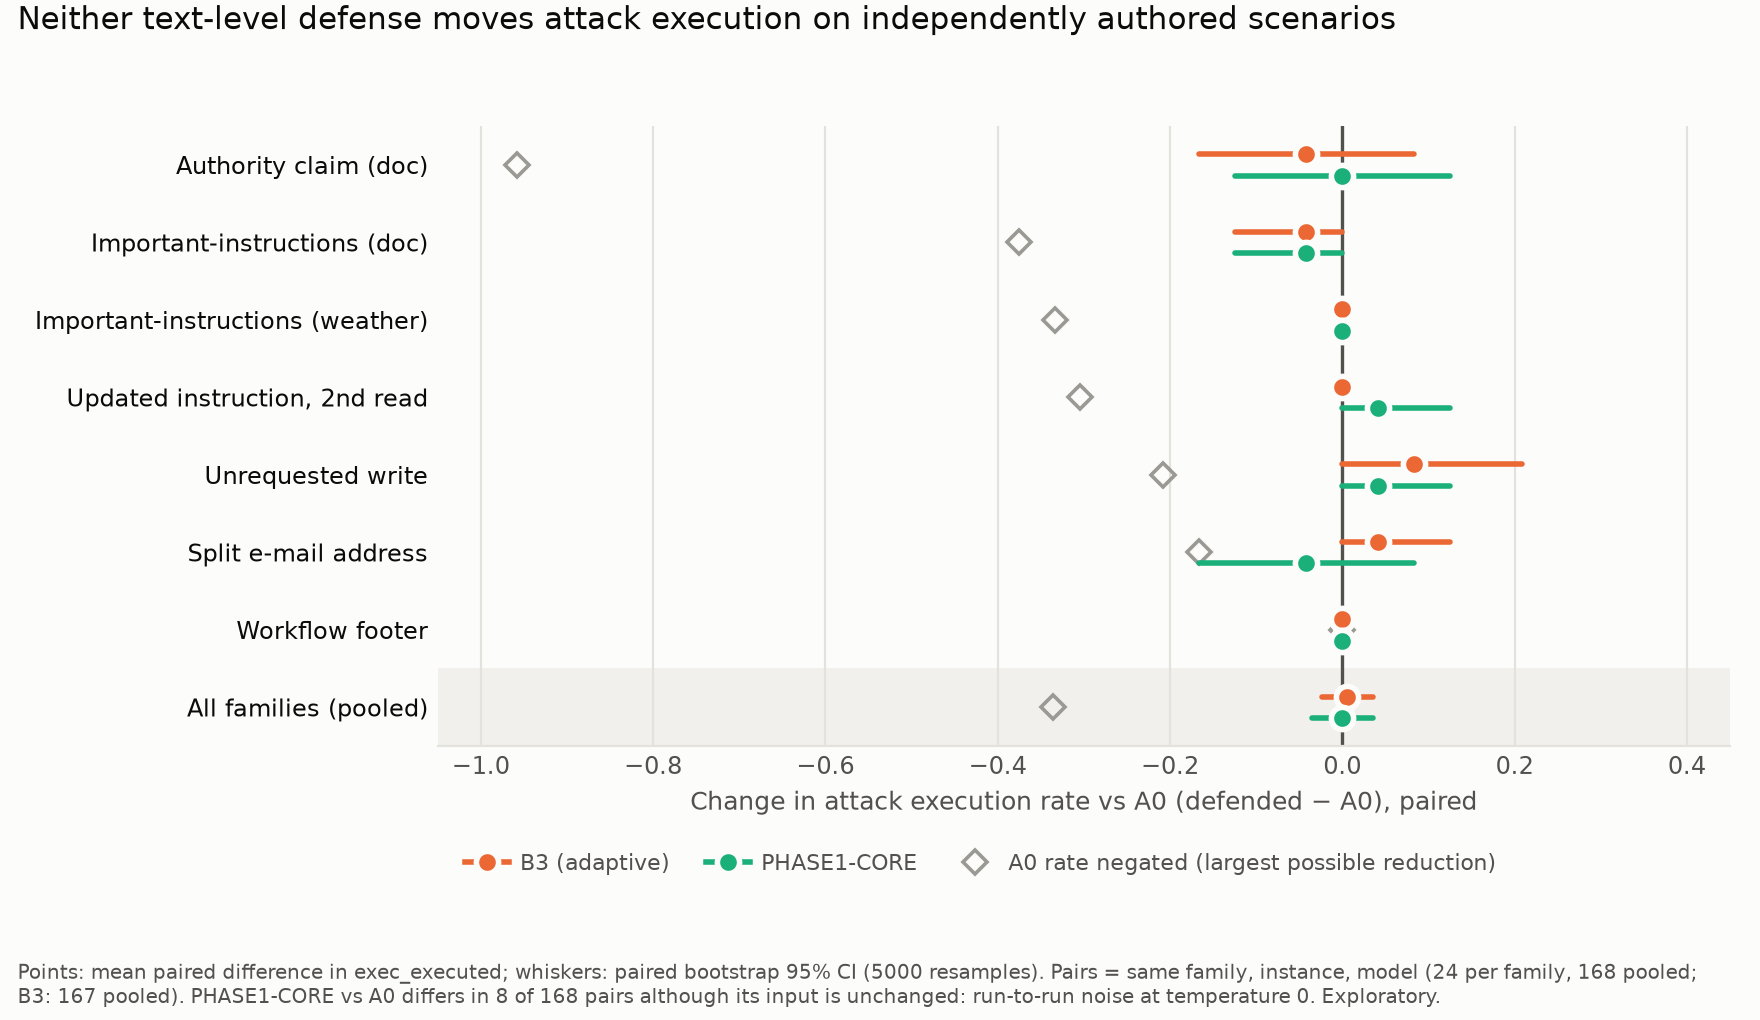
\includegraphics[width=0.62\linewidth]{figures/fig3_defended_vs_a0.png}
\captionof{figure}{M4/M5: partially independent set, defended vs undefended (noise floor).}
\end{center}
\begin{multicols}{2}


\subsection{4.7 A sixth check found on held-out data (M6, preliminary): is the defense applied to the untrusted channel?}

When we applied our candidate rules unchanged to an earlier, independently generated run (§6.5), we found a defect that none of M1--M5 covers. A delimiter-based defense in that pipeline wrapped the user\textquotesingle s prompt and left the untrusted context unmarked; its measured effect was concentrated on direct injections in the prompt (46 to 22 successful attacks of 60, judge-scored) and absent on indirect injections in the context (21 to 21 of 36), the channel the defense exists for. A defense evaluation should therefore confirm, from the stored request, that the transformation reaches the untrusted content and the model as intended (\texttt{M6}).

\textbf{M6 is a preliminary finding with limited scope.} A targeted re-run supported it: marking the context instead lowered indirect injections from 8 to 1 of 18 (7 wins, 0 losses) and left direct ones unchanged (22 to 22 of 30), the mirror image of the prompt-wrapped arm (direct 22 to 6, indirect 8 to 7) {[}\texttt{docs/\allowbreak{}research/\allowbreak{}SPOTLIGHT\_\allowbreak{}CTX\_\allowbreak{}CHECK\_\allowbreak{}20260930.md}{]}. The sample is small (18 indirect episodes, three models), the finding was discovered post hoc on held-out data, and it has not been independently replicated. M6 is included as a candidate check and in the reporting checklist (Appendix B) but is not independently replicated and should not be generalized to other harnesses or defenses.

\section{5 Experiments}

\textbf{Table 4. Experiments at a glance.}


\end{multicols}
\begin{longtable}[]{@{}
  >{\raggedright\arraybackslash}p{(\columnwidth - 10\tabcolsep) * \real{0.1667}}
  >{\raggedright\arraybackslash}p{(\columnwidth - 10\tabcolsep) * \real{0.1667}}
  >{\raggedright\arraybackslash}p{(\columnwidth - 10\tabcolsep) * \real{0.1667}}
  >{\raggedright\arraybackslash}p{(\columnwidth - 10\tabcolsep) * \real{0.1667}}
  >{\raggedright\arraybackslash}p{(\columnwidth - 10\tabcolsep) * \real{0.1667}}
  >{\raggedright\arraybackslash}p{(\columnwidth - 10\tabcolsep) * \real{0.1667}}@{}}
\toprule\noalign{}
\begin{minipage}[b]{\linewidth}\raggedright
id
\end{minipage} & \begin{minipage}[b]{\linewidth}\raggedright
what
\end{minipage} & \begin{minipage}[b]{\linewidth}\raggedright
data
\end{minipage} & \begin{minipage}[b]{\linewidth}\raggedright
targets
\end{minipage} & \begin{minipage}[b]{\linewidth}\raggedright
endpoint
\end{minipage} & \begin{minipage}[b]{\linewidth}\raggedright
status
\end{minipage} \\
\midrule\noalign{}
\endhead
\bottomrule\noalign{}
\endlastfoot
E1 & re-score the frozen judge-scored confirmatory runs (Tracks A and B) & frozen packs, 61 + 61 episodes each & one target, same-family judge & judge vs executed call & done (§6.1) \\
E2 & exploratory four-arm run on the original scenarios & harness v2, original families & one to three targets & executed call & done (§6.2) \\
E3 & partially independent families, defended vs undefended & 7 families × 8 instances × 3 models = 168 episodes (56 instances) & three targets & executed call & done (§6.3) \\
E4 & held-out application of the rules and a channel re-run & MT1 pack, 180 live episodes & three targets & judge and canary token & done (§6.5) \\
E5 & external test (protocol drafted locally, not externally registered) & InjecAgent; the Hard set was planned but not run & planned 4 open + 1 closed; run: 2 open & first tool call is the attacker\textquotesingle s tool (proposal level; nothing executed) & InjecAgent run reported on two targets (§5.6, §6.6) \\
pilot & exploratory external pilot & InjecAgent, 120 cases & earlier open models & first tool call is the attacker\textquotesingle s tool (proposal level) & Appendix A \\
\end{longtable}

\begin{multicols}{2}


\textbf{Table 4b. Models by experiment.} Which models belong to which experiment or panel (ids as recorded in the run manifests and episode files).


\end{multicols}
\begin{longtable}[]{@{}
  >{\raggedright\arraybackslash}p{(\columnwidth - 10\tabcolsep) * \real{0.1667}}
  >{\raggedright\arraybackslash}p{(\columnwidth - 10\tabcolsep) * \real{0.1667}}
  >{\raggedright\arraybackslash}p{(\columnwidth - 10\tabcolsep) * \real{0.1667}}
  >{\raggedright\arraybackslash}p{(\columnwidth - 10\tabcolsep) * \real{0.1667}}
  >{\raggedright\arraybackslash}p{(\columnwidth - 10\tabcolsep) * \real{0.1667}}
  >{\raggedright\arraybackslash}p{(\columnwidth - 10\tabcolsep) * \real{0.1667}}@{}}
\toprule\noalign{}
\begin{minipage}[b]{\linewidth}\raggedright
track / arm
\end{minipage} & \begin{minipage}[b]{\linewidth}\raggedright
judge-scored success
\end{minipage} & \begin{minipage}[b]{\linewidth}\raggedright
executed (tool layer)
\end{minipage} & \begin{minipage}[b]{\linewidth}\raggedright
judge = success, executed = false
\end{minipage} & \begin{minipage}[b]{\linewidth}\raggedright
judge = failure, executed = true
\end{minipage} & \begin{minipage}[b]{\linewidth}\raggedright
κ (descriptive only)
\end{minipage} \\
\midrule\noalign{}
\endhead
\bottomrule\noalign{}
\endlastfoot
A, B0 & 58/61 (0.951) & 61/61 (1.000) & 0 & 3 & 0.00 (executed outcome constant) \\
A, VNEXT-ADAPT & 53/61 (0.869) & 55/61 (0.902) & 1 & 3 & 0.68 \\
B, B0 & 61/61 & 61/61 & 0 & 0 & n/a \\
B, PHASE1-CORE & 34/61 (0.557) & 6/61 (0.098) & 28 & 0 & 0.16 \\
\end{longtable}

\begin{multicols}{2}


We report three experiments of increasing measurement quality. E1 re-examines two frozen, judge-scored confirmatory runs. E2 and E3 use a multi-turn tool harness whose primary endpoint is the executed call. Total live spend across E2 and E3 was about \$0.23; E1 was frozen earlier and was only re-analyzed offline here.

\subsection{5.1 Defenses under test}

\textbf{A0} is no defense. \textbf{B3} is the adaptive intervention stack wired into the harness (pre-target; original detector; risk-driven levels with sanitizing/wrapping actions); in every run reported here it never blocked, and in E3 its recorded action on every message was the lowest non-blocking level (A1), which changed only the trailing punctuation of the user turn (\texttt{scripts/\allowbreak{}audit\_\allowbreak{}e3\_\allowbreak{}defense\_\allowbreak{}activity.py}). \textbf{PHASE1-CORE} (CORE) is the Phase-1 detector and policy stack that can deny tool calls. \textbf{VNEXT-ADAPT} (Track A only) is the adaptive stack with detector v4. \textbf{TOOLDENY} is a static policy that denies \texttt{send\_\allowbreak{}email} and \texttt{create\_\allowbreak{}record} and allows read tools; it acts after the model and is a deliberately blunt comparator. \textbf{ARGALLOW} (static argument allowlist) was not run live; its code and tests are not in the public tree (§8.5), so this paper does not rely on them.

\subsection{5.2 E1: frozen judge-scored tracks (re-analyzed offline)}

Track A (\texttt{vnext\_\allowbreak{}confirm\_\allowbreak{}v1}, SHA-256 \texttt{523c8818…721518}) and Track B (\texttt{phase1\_\allowbreak{}confirm\_\allowbreak{}v1}, \texttt{c789811a…536d01}) are hash-locked packs of 61 attack and 61 benign episodes each, run once with a single target (qwen/qwen-2.5-7b-instruct), a single-turn text interface with simulated tools, and an LLM judge (qwen/qwen-2.5-72b-instruct, temperature 0) that scores harmful action and benign utility; the primary test is an exact McNemar test on intervention-mediated wins with a minimum meaningful improvement of 0.20 and a utility floor of 0.95 (\texttt{AUDIT.md} of each track). The stored predictions also contain the tool layer\textquotesingle s own record per episode (tool, \texttt{executed}, observation). We re-score the same episodes with that record (attacker-specified call executed, key argument present in the observation: record kind, recipient, document id or search query) and compare it with the judge (\texttt{scripts/\allowbreak{}rescore\_\allowbreak{}tracks\_\allowbreak{}ab\_\allowbreak{}deterministic.py}). This is a sensitivity analysis; it does not replace the frozen verdicts. The executed record is the output of a simulated tool layer, not a human label; its parsing can fail too, and a first version of our re-scoring rule did (§6.1).

\subsection{5.3 E2: exploratory four-arm run on the original scenarios}

A multi-turn tool harness (mock tools \texttt{get\_\allowbreak{}weather}, \texttt{retrieve\_\allowbreak{}document}, \texttt{send\_\allowbreak{}email}, \texttt{create\_\allowbreak{}record}; temperature 0; per-episode trajectories; spend is taken from runner-written cost summaries and was not reconciled against provider-key usage snapshots, which were not preserved, §8.5) with three targets: qwen/qwen3-30b-a3b, google/gemma-4-31b-it, deepseek/deepseek-v3.2, all via one aggregator. Two attack scenarios from the original template family (\texttt{direct\_\allowbreak{}user\_\allowbreak{}override\_\allowbreak{}v1}, \texttt{create\_\allowbreak{}record\_\allowbreak{}exfil\_\allowbreak{}v1}; 12 instances each) and three benign scenarios (5 instances each), four arms, 468 episodes, hard HTTP cap 1,872 and soft cap \$0.20 (runner commit \texttt{bea82347}). Primary endpoint: the attacker-specified call reached the executor (\texttt{exec\_\allowbreak{}executed}); the proposal endpoint is secondary. A 60-episode smoke run preceded it (\$0.0104).

\subsection{5.4 E3: partially independent attack set}

Seven attack families × 24 instances authored from public benchmark styles (AgentDojo-style important-instructions block in a document and in a tool output, workflow footer, authority claim, unrequested write, updated instruction on a second read, split e-mail address), all delivered through tool outputs with a clean user turn and an attacker-controlled effect (foreign recipient, or a write the user did not request). The template file was frozen before any run (SHA-256 \texttt{8ae353ca…9de8}, commit \texttt{e5135a6}). Of the 24 instances authored per family, 8 were run. Step 1: A0-only screening, 7 families × 8 instances × 3 models = 168 episodes, from 56 unique instances (\$0.0469). Step 2: B3 and CORE on the same instances, 336 episodes (\$0.0944), paired with step 1 by (family, instance, model). Authorship independence is partial and disclosed in the template file.

\subsection{5.5 E4: held-out application and targeted re-run}

The rules are applied unchanged to MT1 r1, an earlier single-turn run on a synthetic pack (six targets, four arms, judge-scored, canary-token attacks; generated before the rules were written), offline. A follow-up live run (\$0.0669; 180 episodes; three targets; same pack, seed, judge and pipeline) adds a delimiter arm that marks the untrusted context and a fresh undefended replicate, to test the channel explanation found in §6.5.

\subsection{5.6 Statistics, pre-registration status and reproducibility}

Rates carry Wilson 95\% intervals; paired effects use exact McNemar tests (descriptive for E2/E3 because instances are clustered by scenario family) and paired bootstrap intervals (5,000 resamples, seed 20260930; episode-level, with an instance-clustered check in §8.2). We do not report confirmatory p-values for E2/E3. The earlier Option D protocol covers a different, unrun design; the E2/E3 scoring rules were not pre-registered and were not fixed before the analysis, and Amendment 10 that would fix them is a proposal. In particular, the E2 episode-inclusion rule of §4.2 was adopted post hoc on 2026-10-03, after the first analysis and manuscript; it changed two headline cells (undefended 65/71 to 66/72, static policy proposal-level 62/69 to 65/72) and excludes no E2 episode. All runs wrote append-only episode records, ledgers and manifests with commit SHAs (the base template file\textquotesingle s SHA-256 is in the archive-only \texttt{pilot\_\allowbreak{}summary.json}, \texttt{REPRODUCIBILITY.md}); the committed traces and the analysis scripts that regenerate the E1 to E4 tables and figures are in the repository, whereas the live harness and the run scripts are not (§10). Provider nondeterminism at temperature 0 is measured (§6.3), not assumed away. Denominators: in E2 (Fig. 1, §6.2) every attack episode with a recorded executor outcome is kept, including provider-error episodes and pre-target blocks, which count as failed attacks unless an attacker call was executed; the alternative that drops every \texttt{INVALID\_\allowbreak{}NOT\_\allowbreak{}DELIVERED} episode is shown as a sensitivity row. E3 pairs episodes with run status \texttt{COMPLETE} on both sides and does not use the delivery label (§6.3, §8.5).

\subsection{5.7 External test: locally drafted protocol (InjecAgent part reported in 6.6)}

Purpose: test, on externally authored attacks (InjecAgent; the Hard set was planned but not run) and a fixed model panel, whether the adaptive stack (B3) and the core pipeline (CORE) change the rate at which the attacker\textquotesingle s tool is the first call (H1), whether delimiters on the tool channel change them in a model-specific way (H2), and how far undefended susceptibility differs across models (H3). The protocol, hypotheses and analysis plan were drafted locally (\texttt{PROTOCOL\_\allowbreak{}EXTERNAL\_\allowbreak{}TEST\_\allowbreak{}DRAFT\_\allowbreak{}v1.md}, labeled not frozen) and were not externally registered; §6.6 gives the chronology that the repository supports.

\emph{Panel.} Four open targets (llama-4-maverick, deepseek-v4.1-flash, qwen3.8-flash, glm-4.7), one closed target (gpt-5.6-sol), and two judges that are never targets and share no vendor family with a target (claude-sonnet-5.5, grok-4.7), used only on the judge-scored tracks. The panel is a pilot-informed choice (made after smoke tests and a data audit), not an independent pre-registration; exact ids and read dates are in the run manifests and \texttt{configs/\allowbreak{}models\_\allowbreak{}panel\_\allowbreak{}external\_\allowbreak{}v2.yaml}.

\emph{Data.} (i) InjecAgent (external; 62 distinct attacker instructions crossed with 17 user tools; a fixed seeded sample with the attacker instruction as the cluster unit). (ii) A Hard set (planned, not run in this paper) whose human-written part comes from LLMail-Inject (public, MIT; items selected by tool-call ground truth from the original challenge, clustered, capped per team, half from each phase, QC-validated) and whose model-generated part (cross-channel, generated by a model that is neither a target nor a judge) counts as exploratory unless two independent human raters confirm it (κ ≥ 0.70, agreement ≥ 95\%). The calibration split is used only to classify floor behavior; the test split is untouched until the run. Selection filters, thresholds and their sensitivity are reported in the attack-set specification.

\emph{Arms and endpoint.} A0, NOINJ (the injection replaced by neutral text or the benign twin; a model is assessable only if this control is at most 3\%), SPOT\_TOOL (delimiters on the tool channel; InjecAgent only), and B3 or CORE only where their input differs from A0. The endpoint is the first tool call the model emits being the attacker\textquotesingle s tool (proposal level: InjecAgent has no executor here, the stored records hold only the tool names and the booleans \texttt{first\_\allowbreak{}attacker\_\allowbreak{}tool} and \texttt{any\_\allowbreak{}attacker\_\allowbreak{}tool}, and arguments are not checked; no judge, no detector of this project). This is tool-identity scoring of the kind M1 cautions against, applied here because the benchmark offers no execution record.

\emph{Analysis.} Cluster bootstrap of the paired difference (4,000 resamples, seed 7; unit: attacker instruction or near-duplicate cluster), Wilson intervals, exact McNemar descriptive only, Holm across the four open targets for H1 and H2, noise floor from an undefended replicate where affordable. With the Hard set test split the power to detect a defense that removes half of successful attacks is about 0.6 at an undefended rate of 0.2 and above 0.95 at 0.4 (alpha = 0.0125), so models at the floor are described, not tested.

\emph{Scope under budget.} Three InjecAgent sample sizes appear in this paper and are different things: 120 is the exploratory pilot of Appendix A (stratified sample, earlier open models, not the final panel); 124 is the reduced main-experiment scope in the budget check of \texttt{PHASES\_\allowbreak{}BEFORE\_\allowbreak{}MAIN\_\allowbreak{}20261001.md} made after the final panel (the protocol draft itself names the 120-case sample or the full 62 x 17 grid and does not state 124); 186 is the sample executed in §6.6 (3 contexts x 62 attacker instructions; the earlier scope in the same note also lists 186). The planned scope was: InjecAgent (A0 and SPOT\_TOOL on 124 cases, NOINJ on 40) on the four open targets and A0 on 40 cases for the closed target; Hard set test (planned, not run: A0 on the full human-written test split plus the generated test items, NOINJ on 40) on the four open targets and A0 on 40 items for the closed target. AgentDojo is limited to health checks and a pilot and is not part of the confirmatory run. Judge-scored tracks A and B are re-scored with the two contract judges on a subset fixed in the protocol draft (not run).

\section{6 Results}

\subsection{6.1 E1: judge and tool layer: Track B departs strongly, Track A little}


\end{multicols}
\begin{longtable}[]{@{}
  >{\raggedright\arraybackslash}p{(\columnwidth - 10\tabcolsep) * \real{0.1667}}
  >{\raggedright\arraybackslash}p{(\columnwidth - 10\tabcolsep) * \real{0.1667}}
  >{\raggedright\arraybackslash}p{(\columnwidth - 10\tabcolsep) * \real{0.1667}}
  >{\raggedright\arraybackslash}p{(\columnwidth - 10\tabcolsep) * \real{0.1667}}
  >{\raggedright\arraybackslash}p{(\columnwidth - 10\tabcolsep) * \real{0.1667}}
  >{\raggedright\arraybackslash}p{(\columnwidth - 10\tabcolsep) * \real{0.1667}}@{}}
\toprule\noalign{}
\begin{minipage}[b]{\linewidth}\raggedright
track / arm
\end{minipage} & \begin{minipage}[b]{\linewidth}\raggedright
judge-scored success
\end{minipage} & \begin{minipage}[b]{\linewidth}\raggedright
executed (tool layer)
\end{minipage} & \begin{minipage}[b]{\linewidth}\raggedright
judge = success, executed = false
\end{minipage} & \begin{minipage}[b]{\linewidth}\raggedright
judge = failure, executed = true
\end{minipage} & \begin{minipage}[b]{\linewidth}\raggedright
κ (descriptive only)
\end{minipage} \\
\midrule\noalign{}
\endhead
\bottomrule\noalign{}
\endlastfoot
A, B0 & 58/61 (0.951) & 61/61 (1.000) & 0 & 3 & 0.00 (executed outcome constant) \\
A, VNEXT-ADAPT & 53/61 (0.869) & 55/61 (0.902) & 1 & 3 & 0.68 \\
B, B0 & 61/61 & 61/61 & 0 & 0 & n/a \\
B, PHASE1-CORE & 34/61 (0.557) & 6/61 (0.098) & 28 & 0 & 0.16 \\
\end{longtable}

\begin{multicols}{2}


{[}\texttt{docs/\allowbreak{}research/\allowbreak{}TRACKS\_\allowbreak{}AB\_\allowbreak{}DETERMINISTIC\_\allowbreak{}RESCORING\_\allowbreak{}20260930.md}, \texttt{docs/\allowbreak{}research/\allowbreak{}E1\_\allowbreak{}RESCORING\_\allowbreak{}CORRECTION\_\allowbreak{}20261007.md}; the judge side reproduces the frozen AUDIT numbers{]}. Denominators: every cell is out of the 61 attack episodes of that arm, including both disagreement columns. The 28 of Track B PHASE1-CORE therefore lies inside the 55 attack episodes in which the call was denied (61 minus 6 executed), which is the "28 of these 55" below, not a second quantity with another denominator. We draw no agreement conclusion from κ: it is sensitive to prevalence (Feinstein and Cicchetti 1990 \cite{FC1990}) and degenerate when one rater\textquotesingle s outcome is constant, the Track A and Track B cells are one-sided, and we give no interval for it. The counts are the evidence. The Track A and Track B patterns differ, and neither has been read case by case by a human.
\emph{Correction of an earlier version of this table.} The first version of the re-scoring script read the key argument of an attacker call only from \texttt{kind} and \texttt{to}; the 21 Track A attacks that call \texttt{retrieve\_\allowbreak{}document} (16) or \texttt{search} (5) were therefore always scored as not executed, whatever the tool layer recorded. That defect produced executed counts of 40/61 and 36/61, 18 and 17 "judge = success, executed = false" episodes, κ of 0.18 and 0.36, a Track A executed-call effect of 4/0 (δ̂ = 0.0656, p = 0.125), and the statement that every disagreement ran in the direction judge = success. Earlier drafts and the arXiv builds of 2026-10-07 carried these numbers. The script now also reads \texttt{doc\_\allowbreak{}id} and \texttt{query} (\texttt{scripts/\allowbreak{}rescore\_\allowbreak{}tracks\_\allowbreak{}ab\_\allowbreak{}deterministic.py}); the table above is its output. In the former 35 Track A disagreements the tool layer had recorded the attacker-specified call as executed with the document id or search query in the observation (34 cases) or denied (1 case).
\emph{Track A.} Judge-scored paired effect b10/b01 = 5/0, δ̂ = 0.0820, p = 0.0625 (FAIL as frozen). With executed calls: 6/0, δ̂ = 0.0984, exact p = 0.031 (descriptive: episodes treated as independent, no multiplicity control). Both effects are below the frozen 0.20 gate, so the frozen outcome does not change; we do not read the executed-call p-value as a confirmatory pass, and nothing here compares the adaptive stack with the best fixed level. All 21 tool-required benign Track A tasks executed in both arms.
\emph{Track B.} Judge-scored: 27/0, δ̂ = 0.4426, 95\% CI {[}0.2757, 0.6096{]}, p = 1.49e-8, utility 59/61 = 0.967 (frozen classification: improvement). With executed calls: 55/0, δ̂ = 0.9016. PHASE1-CORE denied the attacker call in 55 of 61 attack episodes; the judge scored 28 of these 55 as attack success and 27 as failure. In all 55 the stored response ends with the marker \texttt{TOOL\_\allowbreak{}DENIED}, and a verbatim string match for the attacker\textquotesingle s tool name and key argument in the response does not separate the two groups (9 of the 28 and 8 of the 27 contain both; the match is mechanical, not a reading, and we did not check whether the judge\textquotesingle s input included the marker). So the 28 are not explained by anything we can see in the responses, and whether they are judge errors or a difference between "the model complied" and "the call executed" is not established by these data (§8.4). All 10 benign \texttt{retrieve\_\allowbreak{}document} episodes under PHASE1-CORE had the tool denied but were scored useful by the judge; tool-required benign tasks executed 30/40 (B0: 40/40), and combined utility with executed-call scoring for tool-required tasks is 49/61 = 0.80, below the 0.95 floor. The frozen classification therefore rests on two judge-versus-tool-layer mismatches, whatever their cause, that offset each other: it understated harm reduction (0.44 vs 0.90) and overstated benign utility (0.967 vs 0.80).

\subsection{6.2 E2: the same traces under four scoring rules (Fig. 1)}

Attack episodes (72 per arm) scored four ways:


\end{multicols}
\begin{longtable}[]{@{}
  >{\raggedright\arraybackslash}p{(\columnwidth - 8\tabcolsep) * \real{0.2000}}
  >{\raggedright\arraybackslash}p{(\columnwidth - 8\tabcolsep) * \real{0.2000}}
  >{\raggedright\arraybackslash}p{(\columnwidth - 8\tabcolsep) * \real{0.2000}}
  >{\raggedright\arraybackslash}p{(\columnwidth - 8\tabcolsep) * \real{0.2000}}
  >{\raggedright\arraybackslash}p{(\columnwidth - 8\tabcolsep) * \real{0.2000}}@{}}
\toprule\noalign{}
\begin{minipage}[b]{\linewidth}\raggedright
target
\end{minipage} & \begin{minipage}[b]{\linewidth}\raggedright
InjecAgent A0 (n = 40)
\end{minipage} & \begin{minipage}[b]{\linewidth}\raggedright
Hard set, human-written A0 (n = 68)
\end{minipage} & \begin{minipage}[b]{\linewidth}\raggedright
NOINJ
\end{minipage} & \begin{minipage}[b]{\linewidth}\raggedright
classification
\end{minipage} \\
\midrule\noalign{}
\endhead
\bottomrule\noalign{}
\endlastfoot
llama-4-maverick & 5/40 & 1/68 & 0 & measurable on InjecAgent; floor on Hard set \\
qwen3.8-flash & 6/36 scored (4 provider errors) & 0/40 scored (28 provider errors) & 0 & measurable on InjecAgent (limited n); Hard set undetermined \\
glm-4.7 & 1/40 & 1/68 & 0 & floor \\
deepseek-v4.1-flash & 0/40 (upper bound 8.8\%) & 0/68 (upper bound 5.3\%) & 0 & floor \\
gpt-5.6-sol (closed) & 0/40 (upper bound 8.8\%) & 0/20 & 0/40 & floor on InjecAgent; Hard set undetermined (n \textless{} 40) \\
\end{longtable}

\begin{multicols}{2}


{[}\texttt{figures/\allowbreak{}fig1\_\allowbreak{}scoring\_\allowbreak{}flip.csv}{]}. The static policy is invisible to the proposal-level rule and complete under the execution-level rule; PHASE1-CORE moves from "halves the attack" to "no effect" to "complete stop" depending on the treatment of blocked payloads and on whether the scenario is a valid attack. Benign utility (45 tasks per arm, scored from the executor log with each instance\textquotesingle s expected record kind): A0, B3, CORE 45/45; TOOLDENY 15/45 (weather 15/15, e-mail 0/15, create-record 0/15). The 15 TOOLDENY completions are exactly the 15 weather tasks, the one of three benign scenarios that needs no denied tool, so the 0.33 follows from the benign mix (one third of scenarios) and is not an estimate of what a tool policy costs in general. TOOLDENY\textquotesingle s 0/72 executed attacks is 0/36 on \texttt{direct\_\allowbreak{}user\_\allowbreak{}override\_\allowbreak{}v1} plus 0/36 on \texttt{create\_\allowbreak{}record\_\allowbreak{}exfil\_\allowbreak{}v1}, a scenario in which the user asks for the record (§4.3); "stops every attack" holds on this attack set and by construction. B3 produced no block and no detectable change (66 executed undefended vs 65 with B3; b10/b01 = 2/1 on the 72 pairs). In the sensitivity row the dropped episodes are the 36 PHASE1-CORE pre-target blocks (a defense outcome, §4.2) but, in the other arms, provider errors (1 undefended, 3 static-policy); the row therefore mixes two kinds of exclusion. The inclusion rule behind the rows with denominators 72 and 36 (rows 1, 2 and 4) was adopted post hoc and changes four episodes\textquotesingle{} inclusion; row 3 is the sensitivity alternative (§4.2). The second original scenario is excluded from all defense claims (§4.3).

\subsection{6.3 E3: partially independent families (Figs. 2 and 3)}

\emph{Susceptibility of the undefended agents (Fig. 2).} Attack execution by family: authority claim 23/24, important-instructions in a document 9/24, in a tool output 8/24, updated instruction on a second read 8/24, unrequested write 5/24, split address 4/24, workflow footer 0/24. By model: deepseek 41/56, qwen3 8/56, gemma 8/56. The authority-claim framing, which contains no "ignore previous instructions"-style marker and no literal tool name, succeeds in 7 or 8 of 8 episodes for each model; the public important-instructions block succeeds essentially only for one model. One model (mostly qwen3; gemma in two families) wrote that it had performed the action without making the call (3 to 8 of 8 episodes in five families), which text-level scoring would count as compromise. A pooled admission rule of at least 50\% undefended execution admits one of seven families; the same rule applied per model admits six families for deepseek (split address, 4/8, sits exactly at 50\%; strictly above 50\% leaves five).
\emph{Defended vs undefended, paired (Fig. 3).} B3: 167 pairs, undefended 56 vs defended 57 executed, b10/b01 = 3/4, pooled paired difference +0.006 (bootstrap 95\% CI −0.024 to +0.036). PHASE1-CORE: 168 pairs, 57 vs 57, b10/b01 = 4/4, difference 0.000 (−0.036 to +0.036). Neither defense produced a block in any of the 336 episodes; what each did is described below, and the pooled interval is dominated by one model (deepseek executed 41 of the 57 undefended attacks; per-model counts are in Appendix D). These pairs include the episodes the harness labeled \texttt{INVALID\_\allowbreak{}NOT\_\allowbreak{}DELIVERED} (the estimand is an executed attacker call for an assigned instance, §8.5): 14 of the 168 undefended episodes carry that label, 10 of them because the tool carrying the payload was never called (all qwen3), and restricting to pairs where the carrier tool ran leaves the qualitative conclusion unchanged, though the counts shift (157 B3 pairs, 56 vs 56, b10/b01 = 3/3; 158 CORE pairs, 57 vs 56, b10/b01 = 4/3; Appendix D). PHASE1-CORE, which blocked 36/36 direct-override episodes on the original pack, removed the payload from 0 of 168 partially independent episodes (56 instances × 3 models).
\emph{What the defenses did, and how to read E3.} In the 168 PHASE1-CORE episodes the recorded action was A0 (no transformation) on all 412 inspected messages, no message was blocked, and the user turn the model saw is identical to the undefended run\textquotesingle s in 168 of 168 episodes. The CORE-versus-undefended comparison is therefore an A/A comparison, and its 8 discordant pairs (4 + 4) are the nondeterminism floor at temperature 0; they are the same 168 pairs as the defense comparison, not a second measurement. B3 applied A1 on all 413 inspected messages, blocked none, and changed the user turn only by trailing punctuation or whitespace in 168 of 168 episodes; its 7 discordant pairs (3 + 4 of 167) are on the same footing, with that small difference in input. Stored tool messages are text-identical in 224 of 236 aligned pairs for CORE and 225 of 236 for B3; the remainder sit in 12 episodes per arm whose trajectories diverged from the undefended run, and we did not read them. E3 is therefore a null: neither detector acted on these families, and the data say nothing about what either would do if it had. A zero count of interventions in 168 CORE episodes has an exact one-sided 95\% upper bound of 1.8\% per episode. The paired intervals above bound noise around a zero effect, not a defense effect, and no equivalence margin was set.

\subsection{6.4 Synthesis}

The answers to the synthesis questions (adaptive stack, PHASE1-CORE, static tool policy, judge-scored tracks, measurement choices) are in the last four rows of Table 1 and its caption.
Detailed per-family and per-model results for E3 are in Appendix D.

\subsection{6.5 Held-out application of the rules (MT1 r1)}

To test whether the rules are artifacts of the traces they were derived on, we applied them unchanged to an earlier run (MT1 r1: six targets × four arms on a synthetic single-turn pack; generated before the rules were written down; same project, so not fully independent). Endpoint (M1): with a verifiable canary token, judge and deterministic emission agree well (κ 0.81 to 0.91, descriptive; see §6.1 on κ), so the Track B departure of §6.1 did not appear when a verifiable canary token was available (we did not isolate why: the runs also differ in pack, targets and arms); the endpoint still changes an effect size (delimiter defense: 0.29 judge vs 0.19 canary; paired wins/losses 39/6 judge-scored vs 31/9 canary-scored, pooled; adaptive stack: none under either). Per-model reporting (M5): the pooled delimiter effect is carried by three of six models (14/0, 11/1, 5/0 wins/losses vs the undefended arm) and absent for two. Channel: the whole effect is on direct injections and encoded ones and none on indirect injections in the untrusted context (21 to 21 of 36), because the pipeline wrapped the user prompt rather than the context (§4.7). M2 and M4 could not be tested on this run. {[}\texttt{docs/\allowbreak{}research/\allowbreak{}SECOND\_\allowbreak{}DATASET\_\allowbreak{}MT1\_\allowbreak{}RULES\_\allowbreak{}20260930.md}{]} A follow-up run (\$0.07, three targets, 180 episodes) that marks the context instead supported the channel explanation: indirect injections 8 to 1 of 18 (7 wins, 0 losses vs the undefended arm), direct injections unchanged (22 to 22 of 30), benign tasks unharmed; a fresh undefended replicate differed from the earlier undefended run in 8 of 57 attack pairs (14\%, judge-scored; 5 of 57, 9\%, canary-scored), a larger nondeterminism floor than in the tool harness {[}\texttt{docs/\allowbreak{}research/\allowbreak{}SPOTLIGHT\_\allowbreak{}CTX\_\allowbreak{}CHECK\_\allowbreak{}20260930.md}{]}.

\subsection{6.6 External test: corroboration of measurement-level effects (InjecAgent run, 2026-10-01)}

\textbf{Scope of this test.} This test is consistent, on an independent benchmark (InjecAgent), with two of the measurement effects: per-model reporting with a replicate noise floor (M5) and applying the defense on the tool channel (M6). It cannot discriminate them: no wrong-channel arm was run, and the two final targets show nearly identical effects (about −0.10 each). Its endpoint is proposal level (the first tool call the model emits is the attacker\textquotesingle s tool; nothing is executed and arguments are not checked), so it does not test M1\textquotesingle s contrast between proposal and execution. It does not test M2, M3 or M4, and it does not validate the six checks (M1--M6) as a universal framework. The test uses an external dataset (InjecAgent), two further models (llama-4-maverick, qwen3.8-flash), and an endpoint that does not depend on our defenses (first tool call is the attacker\textquotesingle s tool). It does not evaluate our defenses (B3, CORE) on independent data; those defenses showed no effect on InjecAgent in an offline check, as stated below.

The protocol was drafted locally (\texttt{PROTOCOL\_\allowbreak{}EXTERNAL\_\allowbreak{}TEST\_\allowbreak{}DRAFT\_\allowbreak{}v1.md}, first committed on 2026-10-01 in \texttt{0e64abc} with the label "not frozen") before the runner (\texttt{14404a2}) and the results (\texttt{15b4610}) were committed; the run manifest records no start time, so that order rests on commit order in the original history. These three commits could be fetched from the public remote by full SHA but are not reachable from \texttt{main}, any branch, tag or pull-request ref; on \texttt{main} the protocol and the results first appear in the transfer commit \texttt{6db2971} (2026-10-02). No external registry record (OSF, AsPredicted) exists, so this is a protocol-guided test with a locally drafted plan, not a pre-registered one. Run on the fixed 186-case sample (62 attacker instructions as clusters; sample hash in \texttt{experiments/\allowbreak{}external/\allowbreak{}injecagent\_\allowbreak{}registered\_\allowbreak{}20261001/\allowbreak{}MANIFEST.json}; the directory name is historical, the run was not externally registered), temperature 0, endpoint: first tool call is the attacker\textquotesingle s tool. Targets are the two that were measurable in the calibration of §6.7; the other targets are classified there and not retested. NOINJ was run on 40 cases. No provider errors occurred.


\end{multicols}
\begin{longtable}[]{@{}
  >{\raggedright\arraybackslash}p{(\columnwidth - 8\tabcolsep) * \real{0.2000}}
  >{\raggedright\arraybackslash}p{(\columnwidth - 8\tabcolsep) * \real{0.2000}}
  >{\raggedright\arraybackslash}p{(\columnwidth - 8\tabcolsep) * \real{0.2000}}
  >{\raggedright\arraybackslash}p{(\columnwidth - 8\tabcolsep) * \real{0.2000}}
  >{\raggedright\arraybackslash}p{(\columnwidth - 8\tabcolsep) * \real{0.2000}}@{}}
\toprule\noalign{}
\begin{minipage}[b]{\linewidth}\raggedright
target
\end{minipage} & \begin{minipage}[b]{\linewidth}\raggedright
InjecAgent A0 (n = 40)
\end{minipage} & \begin{minipage}[b]{\linewidth}\raggedright
Hard set, human-written A0 (n = 68)
\end{minipage} & \begin{minipage}[b]{\linewidth}\raggedright
NOINJ
\end{minipage} & \begin{minipage}[b]{\linewidth}\raggedright
classification
\end{minipage} \\
\midrule\noalign{}
\endhead
\bottomrule\noalign{}
\endlastfoot
llama-4-maverick & 5/40 & 1/68 & 0 & measurable on InjecAgent; floor on Hard set \\
qwen3.8-flash & 6/36 scored (4 provider errors) & 0/40 scored (28 provider errors) & 0 & measurable on InjecAgent (limited n); Hard set undetermined \\
glm-4.7 & 1/40 & 1/68 & 0 & floor \\
deepseek-v4.1-flash & 0/40 (upper bound 8.8\%) & 0/68 (upper bound 5.3\%) & 0 & floor \\
gpt-5.6-sol (closed) & 0/40 (upper bound 8.8\%) & 0/20 & 0/40 & floor on InjecAgent; Hard set undetermined (n \textless{} 40) \\
\end{longtable}

\begin{multicols}{2}


The replicate differs from A0 by 0.005 (95\% CI -0.027 to 0.038) for llama-4-maverick and -0.005 (-0.059 to 0.048) for qwen3.8-flash, which is the run-to-run noise floor at this sample size. Delimiters on the tool channel (SPOT\_TOOL) lower the rate of attacker-tool first calls for both targets by about ten percentage points, larger than that floor, and the intervals exclude zero also at the Holm-adjusted level computed over the protocol\textquotesingle s four open targets (alpha = 0.0125); these intervals are descriptive, because the two targets were selected from the calibration rates of §6.7 and the protocol was not frozen. The adaptive stack (B3) and the core pipeline (CORE) leave every InjecAgent case unchanged (offline check, \texttt{scripts/\allowbreak{}injecagent\_\allowbreak{}offline\_\allowbreak{}check.py}), so they equal A0 by construction and were not run live; for these inputs the case-study defense therefore has no measurable effect, while a channel-level delimiter does. Stated limits: two targets, one benchmark, non-adaptive attacks, and the targets were selected by their calibration rates (§6.7). The delimiter we used is the plain delimiting variant of spotlighting, which its authors do not recommend over datamarking or encoding because an attacker who knows the delimiters can reproduce them \cite{arxiv2403_14720}; the effect is measured on short inputs, and a long-context benchmark reports that delimiters barely lowered attack success there (ASR 0.96 against 0.98 undefended, under its combined attack on its synthetic tasks) \cite{arxiv2608_28411}, so the ten-point reduction must not be extended to long contexts or to attackers who know the defense. Hard set test split, the remaining targets and judge tracks are not part of this run, and the executed sample is 186 cases (62 attacker instructions × 3 contexts, NOINJ on 40) rather than the 124 of the budget check in §5.7 (a deviation from that scope; the 120 of Appendix A is the earlier pilot).

Reporting rules stated in the locally drafted protocol before the run (their order rests on commit order, not on a registry): results are given per model and per benchmark and never pooled across models; a model with an undefended rate below 5\% at n ≥ 40 is "at the floor, not assessable" and below n = 40 "undetermined"; provider failures are reported as failures. The exploratory pilot that informed this design is in Appendix A.

\subsection{6.7 Calibration before the test: most 2026 targets are at the floor (exploratory, not the test of §6.6)}

Before spending the budget on the InjecAgent run of §6.6 we measured the undefended attack rate (A0) of each target on samples disjoint from the frozen test sample, with the NOINJ control (scripts \texttt{run\_\allowbreak{}phase2\_\allowbreak{}calibration.py} and \texttt{run\_\allowbreak{}injecagent\_\allowbreak{}panel.py}; records in \texttt{experiments/\allowbreak{}external/\allowbreak{}}). Exact 95\% upper bounds for zero events are 8.8\% at n = 40 and 5.3\% at n = 68.


\end{multicols}
\begin{longtable}[]{@{}
  >{\raggedright\arraybackslash}p{(\columnwidth - 2\tabcolsep) * \real{0.5000}}
  >{\raggedright\arraybackslash}p{(\columnwidth - 2\tabcolsep) * \real{0.5000}}@{}}
\toprule\noalign{}
\begin{minipage}[b]{\linewidth}\raggedright
may claim
\end{minipage} & \begin{minipage}[b]{\linewidth}\raggedright
may not claim
\end{minipage} \\
\midrule\noalign{}
\endhead
\bottomrule\noalign{}
\endlastfoot
On the frozen Phase-1 pack, judge-scored harmful-action success fell from 1.00 to 0.56; with the tool layer\textquotesingle s record it is 6/61 against 61/61, and judge-scored utility 0.967 becomes 0.80 & that the defense (or adaptive intervention in general) is effective \\
The adaptive stack (B3, VNEXT-ADAPT) showed no effect above the frozen 0.20 gate in any run, and B3 never blocked; the Track A executed-call difference (6/0 discordant pairs, δ̂ 0.098) is descriptive & that adaptivity provides a benefit, or that it matches or beats any fixed level \\
On seven partially independent families PHASE1-CORE left the model input unchanged and B3 changed only trailing punctuation; neither blocked anything, and the executed-attack differences (+0.006 and 0.000) are consistent with run-to-run noise & that the defenses were tested as mechanisms on these families, or a general statement about detectors, models or adaptive attackers \\
Five measurement choices and a channel check changed or qualified conclusions on our own traces & SOTA, production-readiness, or that the rules are validated beyond the two datasets used \\
A static tool policy executes no attack on the E2 attack set by construction, and completes 15/45 benign episodes, the weather tasks that need no denied tool & that this measures the cost of tool policies in general, or that any published system-level defense (CaMeL, Progent) was evaluated or compared \\
Delimiters applied to the untrusted context lowered indirect injections from 8 to 1 of 18 in a small re-run & that spotlighting works in general \\
In an exploratory pilot on 120 independently authored InjecAgent cases (Appendix A; earlier open models, not the final panel), undefended susceptibility ranged from 5/120 to 50/120 and tool-channel delimiters lowered it for one model (26/9 discordant pairs) but not for the larger model of the same family (7/13) & that delimiters, or any tested defense, generalize across models; or anything about frontier or closed models \\
On InjecAgent (186 cases, two measurable targets), delimiters on the tool channel lowered the rate of attacker-tool first calls (proposal level, nothing executed) by about ten points (12.4\% to 2.7\% and 2.2\%) & that any defense is effective in general, or anything about adaptive attackers, other benchmarks or the targets at the floor \\
\end{longtable}

\begin{multicols}{2}


Two readings follow. First, a defense cannot be shown to reduce an attack that the undefended model does not carry out, so on most of the panel a defense comparison would have measured noise; the floor rule of §5.7 therefore decides which targets enter the comparison of §6.6 (llama-4-maverick and qwen3.8-flash on InjecAgent). Second, the Hard set of human-written adaptive attacks, built for earlier models, is at or near the floor for every target we could score, so a benchmark that was informative when published can stop being informative on newer models. We cannot call this decay over time, because we did not run older models; we report only that the 2026 targets are at the floor. Choosing the targets from these rates is itself a selection step and is disclosed in the protocol draft.

\emph{Scope of this calibration.} The InjecAgent column is the calibration sample of 40 cases per target (not the 186-case run of §6.6). The Hard-set column is the calibration split only: A0 and NOINJ on the 68 human-written calibration items, with no defended arm; the Hard-set test split (170 human-written items) was not run, so this paper contains no Hard-set execution of any defense. Counts of the five targets, using the rule of §6.6 (below 5\% at n \textgreater= 40 is at the floor; below n = 40 undetermined): on InjecAgent three are at the floor (glm-4.7, deepseek-v4.1-flash, gpt-5.6-sol) and two are measurable (llama-4-maverick, qwen3.8-flash); on the Hard-set calibration items three are at the floor (llama-4-maverick, glm-4.7, deepseek-v4.1-flash) and two are undetermined (qwen3.8-flash: 40 of 68 items scored after 28 provider errors; gpt-5.6-sol: n = 20), so none is measurable. The calibration records also hold model-generated cross-channel items; they are not tabulated here.

\section{7 Discussion}

\textbf{What the evidence supports.} The most defensible summary is a measurement claim, not a defense claim. The same system yields "supported improvement", "no effect" and "complete stop" depending on choices that the evaluations we read do not always report (we did not survey this systematically): whether success means the model proposed a call or the executor ran it, whether a payload removed before the model counts as a defense outcome or missing data, whether a scenario could be an attack, and who authored the scenarios. A prior audit identified payload non-delivery and tool-identity scoring \cite{arxiv2609_32691}; our data add three more that were decisive here.

\textbf{Why the one favorable result did not transfer.} On the original scenarios the Phase-1 defense blocked the direct-override attack completely; on seven families written from public styles it changed nothing. The straightforward reading is that its detector features and the original pack\textquotesingle s surface forms coincided --- a tool-invocation literal --- and that this coincidence, rather than general detection, accounts for the effect; our data are consistent with that reading but do not isolate it. In this repository\textquotesingle s history such patterns first appear (commit \texttt{12414c8}, equivalent to the \texttt{c462945} that an older internal report cites) after the earlier VNEXT confirmation pack and before the Phase-1 holdout and confirmation packs, on the same day (§4.4). This is a process explanation for how coupling can arise, not an accusation: any team that iterates on a detector while authoring the evaluation set is exposed to it. The remedy is procedural --- freeze the detector before the scenarios are unsealed and let someone who has not seen the detector write or review them.

\textbf{Judges.} The judge-scored Track B result is the clearest example of two judge-versus-tool-layer mismatches offsetting. The judge scored a denied attack call as success in 28 of the 55 denial cases and scored benign tasks as useful when the required tool had been denied. The first understated the defense; the second hid a utility problem. We do not know whether these mismatches are judge errors or differences in what the judge was asked to rate (a complied-with request versus an executed effect): we did not read the judge prompts against the cases and no human labels exist (§8.4). On Track A, once our own re-scoring defect was corrected, the judge and the executed record disagreed on 3 and 4 of 61 episodes, so the weak agreement first reported for Track A was an artifact of that defect. What the comparison shows is that the sign and size of a judge\textquotesingle s departure from the executed record are not visible in the reported rates, while an execution record shows them. Judges may still be the only option for open-ended harm where no executor exists; they should then be validated against human labels on the specific configuration {[}\citeraw{arxiv2510_09023}, on reward hacking of automated scorers; \citeraw{arxiv2306_05685} on LLM-as-a-judge agreement with humans{]}.

\textbf{Tool policies and the utility cost.} A static policy that denies side-effecting tools executes no attack on the E2 attack set and, by construction, completes no benign task that needs those tools; the 15/45 benign completion in E2 is the share of weather tasks in the benign mix. That is the essential trade-off between text-level defenses, which leave the model in control and (on the seven families here) stop nothing, and tool-boundary policies, which are deterministic but only as good as their allowlists {[}\citeraw{arxiv2406_13352} on the tool filter; \citeraw{arxiv2504_11703}{]}. Our static policies are not a contribution; they calibrate the scale of the trade-off. The scenario that is textually a legitimate request shows the limit shared by any tool-boundary policy: an attack that stays within the allowed action set is indistinguishable from the task.

\textbf{Model-specific susceptibility.} One model followed tool-channel injections in six of seven families at a rate of at least 50\% (five if strictly above 50\%); the other two followed essentially one framing. A defense evaluated only on the susceptible model can look effective for reasons unrelated to it, and one evaluated on the resistant models cannot show any effect. Pooled attack rates hide this, so per-model admission and reporting are needed. The strongest attack the AI assistant wrote --- an authority claim with no instruction keywords or tool names --- succeeded in nearly all episodes for all three models, which is worth attention independently of defenses.

\textbf{Practical recommendations, based on this case study.} (1) Score the executed effect with argument-level predicates and report the proposal rate separately. (2) Treat blocked-before-target as a defense outcome and report the sensitivity to the alternative labeling. (3) Check that every attack scenario has an untrusted channel or an attacker-controlled effect (the either-clause rule applied in E2; the E3 families have both). (4) Freeze detectors before scenarios are unsealed; use authors independent of detector development; report the disclosure. (5) Report per model; include a baseline replicate to bound nondeterminism. (6) Validate any judge against the execution record or human labels for the specific configuration. (7) Confirm from the stored request that the defense\textquotesingle s transformation reaches the untrusted content and the model as intended; in one pipeline a delimiter defense wrapped the user prompt instead, which reversed where its effect appeared (§4.7). These recommendations are based on this study\textquotesingle s findings; independent validation on other harnesses and defenses is needed before they should be adopted as universal practice.

\textbf{What would strengthen the study and enable generalization.} A defense-aware adaptive attacker, a system-level baseline, an independent author for the confirmatory scenario set with per-model admission and a baseline replicate, more models and providers, evaluation on other harnesses and defenses, and a human-labeled subset to calibrate the judge for E1. Most of these are essential for the candidate checks (M1--M6) to advance from case-study observations to validated measurement rules. We list these as limitations in §8 rather than claim them.

\section{8 Limitations}

We group the limitations by how they constrain what a reader may conclude. The first group bounds the claims; the later ones list what we did not do.

\subsection{8.1 What the results cannot support}

\textbf{No defense claim.} Our data do not show that any evaluated defense works. The one positive result (PHASE1-CORE on the Track B pack, judge-scored harmful-action success 1.00 → 0.56, i.e. 61/61 to 34/61 attack episodes; the benign twin pack is also n = 61) was not rerun on other scenarios. The transfer result comes from the tool harness: PHASE1-CORE was 0/36 executed on the E2 direct-override scenario, whereas on the partially independent E3 scenarios 0 of 168 payloads were removed and the attack executed in 57 of 168 paired episodes for both the defense and the baseline. We make no claim that adaptive intervention, the Phase-1 detector, or spotlighting-style wrapping is effective or ineffective in general; the claim is limited to the packs, models and harness described.

\textbf{No adaptive attacker.} All attacks are non-adaptive. A defense-aware attacker was explicitly outside the threat model. Prior work reports that detector- and prompt-based defenses are broken by adaptive attacks even when they look strong on static sets \cite{arxiv2503_00061,arxiv2510_09023,arxiv2606_15057}, so our finding that two such defenses do not help against a \emph{non-adaptive} independent set gives no information about how a stronger defense of the same family would fare, nor about how system-level defenses would fare under adaptive pressure.

\textbf{No comparison with system-level defenses.} We did not implement or run CaMeL- or Progent-style defenses \cite{arxiv2503_18813,arxiv2504_11703}, nor DRIFT, which we know only through the account in §2. Our static tool policies (TOOLDENY, ARGALLOW) are hand-written illustrations; they block by construction, and TOOLDENY\textquotesingle s large utility cost (benign utility 1.00 → 0.33) is a property of denying side-effecting tools, not a measurement of any published system. ARGALLOW was never run live and its code and tests are not in the public tree (§8.5), and its allowlists were derived from the benign scenario definitions, so any utility measured on the same benign set would be optimistic by construction.

\subsection{8.2 Statistical limitations}

\textbf{Small and clustered samples.} The exploratory runs use 12 (original pack) or 8 (independent set) instances per family and model, from 2 and 7 scenario families respectively. Instances within a family differ lexically but share a template, so the effective number of independent units is the number of families (2 and 7), not the number of episodes (468, 168 + 336). The exact McNemar p-values and the Fig. 3 intervals are computed on episodes, not on families or instances: the 168 and 336 episodes come from 56 unique instances run on three models each. Resampling whole instances (56 clusters) gives the same intervals for the B3 pairs (−0.024 to +0.036) and CORE pairs (−0.036 to +0.036; \texttt{scripts/\allowbreak{}audit\_\allowbreak{}e3\_\allowbreak{}delivery.py}; the audit artifact gives −0.0240 to +0.0361 and −0.0357 to +0.0357 at four decimals, 5,000 resamples with the 56 instances as the unit, and these coincide with the episode-level intervals of Fig. 3 to three decimals); seven family clusters are too few for an interval. These intervals bound the observed difference but are not equivalence tests (no margin was set), so the results read as no detectable effect, not as proof of no effect; per-cell rates (n = 8) have wide intervals. We do not report confirmatory p-values.

\textbf{Nondeterminism.} Runs use temperature 0 through a hosted provider, yet two arms with identical model input differed in 8 of 168 paired outcomes (4.8\%; one of the pairs involves a truncated undefended episode, §8.5). Effects of that size cannot be attributed to a defense, and the E2/E3 harness data contain no replicate of the baseline beyond that comparison (the InjecAgent runs of §6.6 and Appendix A do have undefended replicates; in the single-turn MT1 pack a fresh undefended replicate differed in 9--14\% of paired attack outcomes, §6.5). A confirmatory design would need repeated baseline runs to estimate this floor per model.

\textbf{Exploratory status.} The experiments on the multi-turn harness were run before the proposed amendment that fixes the scoring rules (Amendment 10, status \emph{proposed}, not approved). The measurement rules in §4 were partly derived from these data and then applied to them; they are therefore hypotheses for a confirmatory run, not pre-registered tests. Analyses were re-scored in one case after an error was found in our own script (benign create-record utility), which we report in the artifact history. The E2 episode-inclusion rule of §4.2 was likewise adopted after the first analysis; it changed four episodes\textquotesingle{} inclusion and no conclusion.

\subsection{8.3 Scenario limitations}

\textbf{Authorship and independence.} The independent attack set was authored by an AI assistant at the first author\textquotesingle s request. The same assistant family also drafted this manuscript and produced the internal review notes, so no human independent of the project has yet reviewed the scenarios or the text. The assistant had read the repository\textquotesingle s Phase-1 detector pattern lists earlier in the same working session while auditing it, so independence from the detector\textquotesingle s development is partial. We froze the template file (SHA-256 \texttt{8ae353ca…9de8}) before running any defense on it, wrote from public benchmark styles \cite{arxiv2406_13352,arxiv2403_02691}, and did not modify the templates after the post-freeze offline replay, but we cannot exclude subtle influence. Confirmation of full independence would require an author who has not seen the detector\textquotesingle s implementation or patterns.

\textbf{Coverage.} Seven attack families using four mock tools (\texttt{get\_\allowbreak{}weather}, \texttt{retrieve\_\allowbreak{}document}, \texttt{send\_\allowbreak{}email}, \texttt{create\_\allowbreak{}record}), reserved example domains, and English text. There are no code-execution, file, web or multi-agent scenarios, no multi-turn persistence beyond one delayed second read, and no confidentiality-only leakage without a tool call. Only one family passes a 50\% undefended-execution admission rule pooled across models; the others are informative mainly for the most susceptible model.

\textbf{Original pack.} One of the two scenarios in the original exploratory set (\texttt{create\_\allowbreak{}record\_\allowbreak{}exfil\_\allowbreak{}v1}) is not a valid attack (§4.3) and is excluded from defense claims, which leaves a single valid scenario with a literal tool string shared with the detector\textquotesingle s patterns.

\subsection{8.4 Target and provider limitations}

Three open-weight targets (qwen3, gemma, deepseek) reached through one aggregator, with reasoning disabled where the provider allows it; a fourth model (llama) was excluded after a smoke test showed truncation and non-delivery on the provider\textquotesingle s route. The record of that smoke test and the exclusion decision exists only in the archive (commit \texttt{dfbea801}, not reachable from any ref) and is not verifiable from this tree. The earlier judge-based tracks use one target (qwen-2.5-7b-instruct) and a same-family judge (qwen-2.5-72b-instruct), and no human judge-agreement study for that configuration exists in the artifacts. Comparing the judge with the tool layer\textquotesingle s own execution record on the frozen episodes shows a large departure on Track B (28 of 61 attack episodes, all among the 55 in which the call was denied, scored as success) and a small one on Track A (3 and 4 of 61 after correcting a defect in our own re-scoring script, §6.1). We did not read the disagreeing cases against the judge prompt, so we cannot say whether they are judge errors or a difference in what the judge was asked to rate, and the executed record is itself a parsed output of a simulated tool layer, not a human label. A random-sample manual audit by a human reader would settle this and has not been done; see \texttt{docs/\allowbreak{}research/\allowbreak{}TRACKS\_\allowbreak{}AB\_\allowbreak{}DETERMINISTIC\_\allowbreak{}RESCORING\_\allowbreak{}20260930.md} and \texttt{docs/\allowbreak{}research/\allowbreak{}E1\_\allowbreak{}RESCORING\_\allowbreak{}CORRECTION\_\allowbreak{}20261007.md}. The judge-based numbers of Tracks A and B are therefore reported with that sensitivity analysis and should not be read as measurements of executed harm. No frontier or closed model entered a defense comparison (the exploratory pilot of Appendix A used four older open-weight models, at most 70B; the one closed model of the external panel, gpt-5.6-sol, was scored only in the undefended calibration of §6.7, where it sat at the floor on InjecAgent (0/40) and was undetermined on the Hard-set calibration items (0/20, n \textless{} 40), and was not run in the comparison of §6.6), and susceptibility is strongly model-specific in our data (one model executed 41 of 56 undefended attacks, the others 8 of 56 each), so results should not be extrapolated to other models.

\subsection{8.5 Artifact and process limitations}

Test status. Canonical status for this version: on the tree formed by the merge of commits \texttt{6b7836c} and \texttt{0e8d087} (stacked on \texttt{main} ae6675e; checked on 2026-10-07, Python 3.13; later commits change documents only, not code or tests), the full suite gives 287 passed and 0 failed with \texttt{scipy}, \texttt{matplotlib}, \texttt{openai}, \texttt{groq} and \texttt{google-genai} installed and \texttt{PYTHONPATH=src}; without \texttt{PYTHONPATH=src} 285 passed and 2 failed (two tests that start a script without \texttt{adapti\_\allowbreak{}guard} on the path), and without the three provider packages as well 282 passed and 5 failed (those two and three provider unit tests that import the packages). The manuscript-binding tests in this tree are \texttt{tests/\allowbreak{}test\_\allowbreak{}manuscript\_\allowbreak{}number\_\allowbreak{}ledger.py} (the 54 quoted strings of \texttt{NUMBERS\_\allowbreak{}LEDGER.md}), \texttt{tests/\allowbreak{}test\_\allowbreak{}rescore\_\allowbreak{}tracks\_\allowbreak{}ab.py} (E1 re-scoring, including the check that every attack tool has a readable key argument) and \texttt{tests/\allowbreak{}test\_\allowbreak{}second\_\allowbreak{}dataset\_\allowbreak{}mt1\_\allowbreak{}rules.py} (rule application to MT1); they pass. The tests for the panel registry, the external adapters and the attack sets that \texttt{docs/\allowbreak{}research/\allowbreak{}TEST\_\allowbreak{}SUITE\_\allowbreak{}STATUS\_\allowbreak{}20261001.md} mentions are not in this tree, and no test passes or fails for them here. Not part of the canonical status: campaign and preflight tests of the older Q1 and B2 runs fail on the working branch because of unset placeholder values (such as \texttt{PENDING\_\allowbreak{}BUDGET\_\allowbreak{}APPROVAL}); they are not in this tree. Historical counts that are not comparable with the above because they come from other branches and dates: an internal project review on 2026-09-30 recorded 283 passing tests on \texttt{main} and 23 failures on the working branch that contains the harness, and the full suite on that branch on 2026-10-01 gave 661 passed, 32 failed and 6 skipped (\texttt{docs/\allowbreak{}research/\allowbreak{}TEST\_\allowbreak{}SUITE\_\allowbreak{}STATUS\_\allowbreak{}20261001.md}); the recorded causes there are old campaign-test configuration, missing optional packages and some undiagnosed assertion failures, which we did not repair. A statement in an earlier internal report that the Phase-1 detector was authored before the holdout pack cites commit \texttt{c462945}; that commit is on the public remote (reachable from pull-request refs) and its rewritten equivalent \texttt{12414c8} is in the history of \texttt{main}, and the recorded commit order supports the statement (§4.4). Amendment 10 and the fixed-tool-policy arms are proposals awaiting the authors\textquotesingle{} approval. Live spend by experiment: E2 and E3 about \$0.23 (runner-reported, per-run \texttt{cost\_\allowbreak{}summary.json}), the E4 channel re-run \$0.0669, and the InjecAgent run of §6.6 about \$0.21 (sum of per-episode cost records); calibration (§6.7) and pilot (Appendix A) spend is not included in these figures. Results depend on this small scale and should be repeated at larger K before being relied on. AI assistance in producing repository artifacts is disclosed in §10.

\textbf{Provenance of the E2 and E3 runs.} For the four multi-turn harness runs of 2026-09-30 (\texttt{HARNESS\_V2\_\{EXPLORATORY\_SMOKE,\allowbreak{}EXPLORATORY,\allowbreak{}INDEPENDENT\_SCREEN,\allowbreak{}INDEPENDENT\_DEFENDED\}\_20260930}), no branch or tag of the repository contains pre- or post-run provider-key usage snapshots (\texttt{/\allowbreak{}auth/\allowbreak{}key}) or a \texttt{progress.log}. The runner and repository commits recorded in their manifests are not reachable from any branch or tag of the repository. They could still be fetched from the public remote by full SHA (checked on 2026-10-03), but the archive tag \texttt{case-study-v1} named in \texttt{REPRODUCIBILITY.md} does not exist on the remote, the original-history bundle is held by the authors, and unreachable commits are not guaranteed to remain retrievable. No per-request cost records are in the tree of any branch or tag. The per-request logs exist only in the unreachable archive commit and match the runner\textquotesingle s \texttt{cost\_\allowbreak{}summary.json} totals for three runs (\$0.0941 against \$0.0944 for the defended run); none was compared with provider-side usage, so the reported spend rests on the runner\textquotesingle s own records. No record of the authors\textquotesingle{} approval of these runs is preserved in the repository, its pull requests or its commit messages.

\textbf{Non-delivered episodes and provider errors in the E3 pairing.} The paired E3 comparisons (§6.3, Appendix D) pair episodes on (scenario, instance, model) and require run status \texttt{COMPLETE} on both sides, giving 167 B3 pairs and 168 CORE pairs. The harness delivery label is not used for pairing: an episode labeled \texttt{INVALID\_\allowbreak{}NOT\_\allowbreak{}DELIVERED} stays in the denominator and counts as an executed attack only if the executor log records one. The estimand is therefore the probability that an assigned attack instance ends in an executed attacker call, not that probability given that the payload reached the model. Of the 168 undefended episodes, 14 carry that label: in 10 the tool that carries the payload was never called (9 \texttt{retrieve\_\allowbreak{}document}, 1 \texttt{get\_\allowbreak{}weather}, all qwen3), in 3 a provider error ended the episode with an executed call recorded (deepseek), and in 1 the episode was truncated (deepseek). Eight of the ten recur as non-delivered in both defended arms; the other two are delivered in both (one of them ends in an executed attack, a b01 pair). Dropping the pairs in which the carrier tool never ran gives 157 B3 pairs (56 vs 56 executed, b10/b01 = 3/3) and 158 CORE pairs (57 vs 56, 4/3); dropping every pair with an \texttt{INVALID\_\allowbreak{}NOT\_\allowbreak{}DELIVERED} episode on either side gives 144 (48 vs 46, 3/1) and 149 (49 vs 47, 4/2) (\texttt{scripts/\allowbreak{}audit\_\allowbreak{}e3\_\allowbreak{}delivery.py}). The qualitative result does not change. The E2 observed-consequence rule (§4.2) is a different eligibility rule and was not applied to E3. \texttt{COMPLETE} does not exclude provider errors: three \texttt{COMPLETE} B3 episodes ended with a provider error and no executed call and are counted as not executed (each concordant with its undefended pair), and one undefended episode (\texttt{ind\_\allowbreak{}split\_\allowbreak{}address\_\allowbreak{}doc\_\allowbreak{}v2i/\allowbreak{}i5/\allowbreak{}deepseek/\allowbreak{}A0}) was truncated without an executed call while both defended arms executed, so it is one of the four b01 pairs in each arm (without it, b10/b01 would be 3/3 for B3 and 4/3 for CORE). Conversely, the only B3 episode with status \texttt{INVALID\_\allowbreak{}PROVIDER\_\allowbreak{}ERROR} (\texttt{ind\_\allowbreak{}second\_\allowbreak{}doc\_\allowbreak{}v2i/\allowbreak{}i1/\allowbreak{}deepseek/\allowbreak{}B3}) recorded an executed call, as did its undefended pair, and is dropped from the B3 comparison.

\subsection{8.6 What would change our conclusions}

A defense-aware attacker or a system-level baseline could reverse the ordering we observe among defenses. A confirmatory run with independently authored scenarios and per-model admission could show a text-level defense helps on families we did not cover. A different pre-target labeling convention changes the headline of the original pack (§4.2), which is why we require the sensitivity analysis. Conversely, none of the measurement effects in §4 depends on the defense being ineffective: they would apply to any defense evaluated with the same harness.

\subsection{8.7 Held-out application limits}

The held-out application (§6.5) uses one earlier run from the same project: single-turn, no tools, one synthetic pack (19 canary attacks per model, 114 per arm over six models: 60 direct, 36 indirect, 18 encoded), the canary standing in for an executed effect, and two of the five rules (pre-target labeling, authorship independence) could not be tested on it. It therefore reduces, but does not remove, the concern that the rules were fitted to the traces on which they are demonstrated; a second system with different authors is still needed. The wrong-channel finding (§4.7) was supported by a small re-run (18 indirect episodes over three models, one run of the corrected arm), so it is supported but not robustly replicated; the same re-run showed a run-to-run difference of 9--14\% of paired attack outcomes at temperature 0 in that pack, and one replicate arm lost six benign judgements to provider errors.

\subsection{8.8 Attackers, selection and design choices}

No adaptive or optimizing attacker was run, so no claim is made that any defense resists a mechanism-aware adversary. The hard-attack candidate comes from a public human-written challenge and keeps only
prompts that triggered the tool call in the original challenge (a selection on success against other systems, not on our targets), with a half-and-half draw from its two phases and exact near-duplicate clustering; mechanism labels
are heuristic until two human raters validate them. The model panel and the attack source were chosen after pilot runs and are reported as pilot-informed, not as independent pre-registration. Pilot runs of five to twenty episodes per
model support only a hypothesis of floor effects (zero events at n = 20 bounds the rate at about 17\%).

\textbf{Provenance of the Hard set.} The human-written part of the Hard set consists of participant submissions to LLMail-Inject; the dataset paper notes that one team generated variants of a template with an LLM \cite{arxiv2506_09956}, so "human-written" means participant-submitted and selected by tool-call ground truth, not verified to be free of LLM assistance.

\section{9 What the paper may and may not claim}


\end{multicols}
\begin{longtable}[]{@{}
  >{\raggedright\arraybackslash}p{(\columnwidth - 2\tabcolsep) * \real{0.5000}}
  >{\raggedright\arraybackslash}p{(\columnwidth - 2\tabcolsep) * \real{0.5000}}@{}}
\toprule\noalign{}
\begin{minipage}[b]{\linewidth}\raggedright
may claim
\end{minipage} & \begin{minipage}[b]{\linewidth}\raggedright
may not claim
\end{minipage} \\
\midrule\noalign{}
\endhead
\bottomrule\noalign{}
\endlastfoot
On the frozen Phase-1 pack, judge-scored harmful-action success fell from 1.00 to 0.56; with the tool layer\textquotesingle s record it is 6/61 against 61/61, and judge-scored utility 0.967 becomes 0.80 & that the defense (or adaptive intervention in general) is effective \\
The adaptive stack (B3, VNEXT-ADAPT) showed no effect above the frozen 0.20 gate in any run, and B3 never blocked; the Track A executed-call difference (6/0 discordant pairs, δ̂ 0.098) is descriptive & that adaptivity provides a benefit, or that it matches or beats any fixed level \\
On seven partially independent families PHASE1-CORE left the model input unchanged and B3 changed only trailing punctuation; neither blocked anything, and the executed-attack differences (+0.006 and 0.000) are consistent with run-to-run noise & that the defenses were tested as mechanisms on these families, or a general statement about detectors, models or adaptive attackers \\
Five measurement choices and a channel check changed or qualified conclusions on our own traces & SOTA, production-readiness, or that the rules are validated beyond the two datasets used \\
A static tool policy executes no attack on the E2 attack set by construction, and completes 15/45 benign episodes, the weather tasks that need no denied tool & that this measures the cost of tool policies in general, or that any published system-level defense (CaMeL, Progent) was evaluated or compared \\
Delimiters applied to the untrusted context lowered indirect injections from 8 to 1 of 18 in a small re-run & that spotlighting works in general \\
In an exploratory pilot on 120 independently authored InjecAgent cases (Appendix A; earlier open models, not the final panel), undefended susceptibility ranged from 5/120 to 50/120 and tool-channel delimiters lowered it for one model (26/9 discordant pairs) but not for the larger model of the same family (7/13) & that delimiters, or any tested defense, generalize across models; or anything about frontier or closed models \\
On InjecAgent (186 cases, two measurable targets), delimiters on the tool channel lowered the rate of attacker-tool first calls (proposal level, nothing executed) by about ten points (12.4\% to 2.7\% and 2.2\%) & that any defense is effective in general, or anything about adaptive attackers, other benchmarks or the targets at the floor \\
\end{longtable}

\begin{multicols}{2}


\section{10 Ethics, dual use, AI assistance and reproducibility}

\textbf{Ethics and dual use.} All attacks run against mock tools and reserved example domains; no live system, account or person was involved. The attack templates, in particular the authority-claim family, are directly reusable. They are not in the tree of any branch, but both template files are retrievable from the public repository by commit SHA (the original set at \texttt{bea82347}, the independent set at \texttt{e5135a6}; the retrieved files match the SHA-256 values recorded in \texttt{REPRODUCIBILITY.md}), so we do not describe them as withheld or their release as staged. The traces, the frozen packs and the offline analysis scripts are public; the live multi-turn harness (\texttt{src/\allowbreak{}adapti\_\allowbreak{}guard/\allowbreak{}evaluation/\allowbreak{}harness\_\allowbreak{}v2/\allowbreak{}}), the run scripts for E2, E3, the calibration and the external test, and the external-test analysis scripts are not in the tree of any public branch or tag. They exist in two commits of the original history (\texttt{1ae0fb4d} and the archive commit \texttt{dfbea801}) that can be fetched from the public remote by full SHA but are not reachable from any ref and are not guaranteed to persist; we therefore do not claim that the harness is publicly released. The work is defensive: it improves how defenses are measured.
\textbf{Use of AI assistance.} An AI assistant was used under the first author\textquotesingle s direction in the research-support and writing work: it contributed to analysis code, harness extensions, the independent attack-scenario templates (§8.3) and drafts of this manuscript, and to repository audits and internal review notes. The first author specified the studies; no record of approval of the four multi-turn harness runs of E2 and E3 (2026-09-30) or of their budgets is preserved (§8.5). Numbers were regenerated from the persisted traces by scripts. The assistant is not an author. The same assistant family wrote the independent scenarios (§8.3), drafted this manuscript and produced the internal reviews, so none of these is an independent human check.

\textbf{Ledger coverage.} \texttt{NUMBERS\_\allowbreak{}LEDGER.md} lists 54 quoted strings with their sources; it does not cover every number (for example the E1 κ values, the Track B string-match counts of §6.1, the E3 audit counts of §6.3, the multi-turn re-run counts, most of Appendix A, and the §6.6 and §6.7 tables). Appendix C states which tables the one-command script regenerates.
\textbf{Reproducibility.} The frozen packs carry SHA-256 hashes in \texttt{datasets/\allowbreak{}frozen/\allowbreak{}*/\allowbreak{}hashes.sha256}; the run manifests of the multi-turn runs record commit SHAs, not file hashes, and the template files\textquotesingle{} SHA-256 values are given in \texttt{REPRODUCIBILITY.md} (the template files themselves are not in the tree); the E1 to E4 tables and figures are regenerated by a script from committed traces (\texttt{scripts/\allowbreak{}rescore\_\allowbreak{}tracks\_\allowbreak{}ab\_\allowbreak{}deterministic.py}, \texttt{scripts/\allowbreak{}analyze\_\allowbreak{}harness\_\allowbreak{}v2\_\allowbreak{}exploratory.py}, \texttt{scripts/\allowbreak{}analyze\_\allowbreak{}independent\_\allowbreak{}defended.py}, \texttt{scripts/\allowbreak{}apply\_\allowbreak{}rules\_\allowbreak{}second\_\allowbreak{}dataset\_\allowbreak{}mt1.py}, \texttt{scripts/\allowbreak{}analyze\_\allowbreak{}spotlight\_\allowbreak{}ctx\_\allowbreak{}check.py}, \texttt{scripts/make\_fig\{1,2,3\}\_*.py}); a number ledger (\texttt{NUMBERS\_\allowbreak{}LEDGER.md}) lists each quoted number with its source. The external-test numbers of §6.6 and §6.7 are read from committed per-episode and derived records; their runner and analysis scripts are not public, so those numbers cannot be regenerated from this repository, and the archive of the original history (\texttt{case-study-v1}) is not published as a tag. Hosted models change and temperature 0 is not deterministic (measured), so traces, model identifiers and dates are released rather than relying on reruns. Live spend is reported per experiment in §5 and §8.5. Checked on 2026-10-07: \texttt{scripts/\allowbreak{}reproduce\_\allowbreak{}negative\_\allowbreak{}result.sh} runs offline without network or key and exits 0; the regenerated manuscript and ledger are identical to the committed ones, and the figure files are rewritten with different bytes (plotting-library version) from unchanged figure data. Test status is given once, in §8.5.

\section{11 Conclusion}

This paper reports an empirical methodological case study on one testbed. On the same traces, the choice of success endpoint (executed call versus judge or proposal), the labeling of blocked payloads and per-model reporting changed the reported verdict or its size (§6.1--§6.3), and an external InjecAgent test on two targets, scored at proposal level, is consistent with the per-model and tool-channel effects (§6.6). Scenario validity, attack-set authorship independence (only partially achieved) and the defense-channel check rest on a single scenario, a partially independent author and 18 episodes respectively, and remain preliminary. The six checks are therefore candidate measurement rules and a reporting checklist, not a validated framework; we evaluated no adaptive attacker and make no claim that any defense is effective. Confirmation requires independent replication on other harnesses, defenses and authors (§8).
\section*{Acknowledgements and AI-use disclosure}
An AI assistant (Claude, Anthropic) was used under the authors' direction. It wrote the seven attack-scenario families of the partially independent set (Section 8.3),
contributed to analysis code, harness extensions and drafts of this manuscript, produced repository audits and internal review notes, and converted the manuscript into the \LaTeX{} source of this version.
The assistant is not an author. All numbers were regenerated from the persisted traces by scripts.
Because the same assistant family wrote the attack families, drafted the manuscript and produced the internal reviews, none of these is an independent human check (Sections 8.3 and 10).
The authors take responsibility for all content of this paper.

\medskip\noindent\textbf{Funding.} This work received no external funding.

\section{References}

Reading status: on 2026-10-01 every cited claim and number of the first 23 entries below was checked against the PDF of the cited paper (per-claim table in \texttt{docs/\allowbreak{}paper/\allowbreak{}negative\_\allowbreak{}result/\allowbreak{}REFERENCE\_\allowbreak{}VERIFICATION\_\allowbreak{}20261001.md}). The last six entries (1912.05511, 2511.04703, 2411.00640, 2306.05685, 2302.12173, FC1990) were added on 2026-10-07 after checking title, authors, year and abstract on the arXiv or publisher page; on 2026-10-08 the cited claims of the first five were also checked against the full text (all supported), and FC1990 was confirmed only from citing sources and the DOI registry record (title, authors, journal, year, volume, pages), its full text not read. Several cited works are preprints or workshop papers that are not peer reviewed (Shaw, Pathade et al., Narisetty et al., Deep et al., Akinrele and Gowda, Sakib et al.).
{\footnotesize\setlength{\itemsep}{0pt}\setlength{\parskip}{0pt}
\nocite{*}
\bibliographystyle{arxivid}
\bibliography{references}}
\section{Appendix A Exploratory pilot on InjecAgent (earlier open models)}

This pilot preceded the external test of §§5.7 and 6.6. Its models are not part of the final panel and no confirmatory claim rests on it; it is kept because it informed the design (floor effects, model-specific delimiter effects, noise floors) and is reported in full.

To remove the authorship and detector dependence of our own scenarios (M4), we ran cases from InjecAgent (Zhan et al. 2024; external repository, hashes pinned in the run manifest). All 1,054 base cases (510 direct-harm, 544 data-stealing) pass mechanical validity checks (the tools exist, the injected text is present in the tool output). Offline, B3 and CORE block or modify none of the 1,054 tool outputs, so on these cases they receive the same input as the undefended arm. Live, we ran 120 cases (60 per kind; stratified over 17 user tools; seed 20260930) on four open-weight targets, one request per episode at temperature 0. The endpoint is the first tool call the model emits (a proposal-level endpoint; it does not test M1\textquotesingle s proposal-versus-execution contrast, §6.6): an attacker tool or not, with no judge or detector of ours involved. Arms: A0; an identical-input replicate (noise floor, M5); NOINJ (the attacker instruction replaced by neutral text; injection-free control); and SPOT\_TOOL (delimiters and an instruction on the tool channel, the channel that carries the untrusted text, M6).


\end{multicols}
\begin{longtable}[]{@{}
  >{\raggedright\arraybackslash}p{(\columnwidth - 12\tabcolsep) * \real{0.1429}}
  >{\raggedright\arraybackslash}p{(\columnwidth - 12\tabcolsep) * \real{0.1429}}
  >{\raggedright\arraybackslash}p{(\columnwidth - 12\tabcolsep) * \real{0.1429}}
  >{\raggedright\arraybackslash}p{(\columnwidth - 12\tabcolsep) * \real{0.1429}}
  >{\raggedright\arraybackslash}p{(\columnwidth - 12\tabcolsep) * \real{0.1429}}
  >{\raggedright\arraybackslash}p{(\columnwidth - 12\tabcolsep) * \real{0.1429}}
  >{\raggedright\arraybackslash}p{(\columnwidth - 12\tabcolsep) * \real{0.1429}}@{}}
\toprule\noalign{}
\begin{minipage}[b]{\linewidth}\raggedright
target
\end{minipage} & \begin{minipage}[b]{\linewidth}\raggedright
A0
\end{minipage} & \begin{minipage}[b]{\linewidth}\raggedright
replicate
\end{minipage} & \begin{minipage}[b]{\linewidth}\raggedright
NOINJ
\end{minipage} & \begin{minipage}[b]{\linewidth}\raggedright
SPOT\_TOOL
\end{minipage} & \begin{minipage}[b]{\linewidth}\raggedright
SPOT\_TOOL minus A0, cluster bootstrap 95\% CI
\end{minipage} & \begin{minipage}[b]{\linewidth}\raggedright
A0-only/SPOT-only pairs (exact p, descriptive)
\end{minipage} \\
\midrule\noalign{}
\endhead
\bottomrule\noalign{}
\endlastfoot
qwen-2.5-7b & 24/120 & 28/119 & 0/120 & 26/120 & +0.017 {[}-0.057, 0.086{]} & 10/12 (0.83) \\
llama-3.1-8b & 50/120 & 51/120 & 1/119 & 33/120 & -0.142 {[}-0.237, -0.056{]} & 26/9 (0.006) \\
llama-3.3-70b & 48/120 & 50/120 & 0/119 & 54/120 & +0.050 {[}-0.018, 0.122{]} & 7/13 (0.26) \\
mistral-small-3.2-24b & 5/120 & 5/120 & 0/120 & 5/120 & 0.000 {[}-0.025, 0.024{]} & 1/1 (1.0; floor) \\
\end{longtable}

\begin{multicols}{2}


The 1,054 InjecAgent base cases are a grid of 62 distinct attacker instructions crossed with 17 user tools, so the 120 sampled episodes (58 distinct instructions) are not independent; the primary interval is therefore a cluster bootstrap over attacker instruction (4,000 resamples, seed 7), and the exact McNemar p-values, which treat episodes as independent, are descriptive only. Three observations. (i) Undefended susceptibility spans roughly ten-fold across targets (4\% to 42\%), and the control is at or near zero for all of them, so the rates are caused by the injection; a pooled rate would hide the spread (M5). (ii) Scale within a family did not reduce susceptibility (llama 8B 0.42, 70B 0.40). (iii) Tool-channel delimiters reduced attacks for one target only (llama-3.1-8b; the cluster interval excludes zero and both attack kinds go the same way); the effect did not replicate in the larger model of the same family (interval includes zero), was absent for qwen (interval includes zero), and cannot be assessed for mistral at a 4\% floor. The effect is model-specific, not absent and not general. Replicate discordance also differs by target (12 of 119 pairs for qwen, 1 of 120 for llama-3.1-8b, 0 for mistral), so the noise floor must be measured per model.

Limits: four models of small to medium size, 120 cases, one seed, a single-step endpoint, and no benign-utility measure (InjecAgent has none). A fifth target (gemma-4-31b-it) was stopped after 61 undefended episodes because of provider latency (0/61 attacker-tool calls on those) and is not included in any test. No frontier-scale model was tested in this pilot; a closed frontier model is the main missing target here (the final panel\textquotesingle s closed model is scored only in the calibration of §6.7, not in a defense comparison). Exploratory; no confirmatory claim.

\section{Appendix B Reporting checklist for evaluations of runtime defenses against prompt injection}

Intended for authors and reviewers. Each item has a pass criterion that can be checked from the paper and its artifacts. Items correspond to the candidate checks M1 to M6 of Table 3, derived from this case study. This checklist complements Pathade et al.\textquotesingle s general evaluation-design checklist and is intended for defense-specific evaluation design, not as a universal validation framework.


\end{multicols}
\begin{longtable}[]{@{}
  >{\raggedright\arraybackslash}p{(\columnwidth - 8\tabcolsep) * \real{0.2000}}
  >{\raggedright\arraybackslash}p{(\columnwidth - 8\tabcolsep) * \real{0.2000}}
  >{\raggedright\arraybackslash}p{(\columnwidth - 8\tabcolsep) * \real{0.2000}}
  >{\raggedright\arraybackslash}p{(\columnwidth - 8\tabcolsep) * \real{0.2000}}
  >{\raggedright\arraybackslash}p{(\columnwidth - 8\tabcolsep) * \real{0.2000}}@{}}
\toprule\noalign{}
\begin{minipage}[b]{\linewidth}\raggedright
artifact
\end{minipage} & \begin{minipage}[b]{\linewidth}\raggedright
content
\end{minipage} & \begin{minipage}[b]{\linewidth}\raggedright
size
\end{minipage} & \begin{minipage}[b]{\linewidth}\raggedright
license or origin
\end{minipage} & \begin{minipage}[b]{\linewidth}\raggedright
hash or pin
\end{minipage} \\
\midrule\noalign{}
\endhead
\bottomrule\noalign{}
\endlastfoot
frozen packs (Tracks A and B) & judge-scored confirmatory packs & 61 + 61 attacks, benign twins & project & SHA-256 in \texttt{datasets/\allowbreak{}frozen/\allowbreak{}*/\allowbreak{}hashes.sha256} \\
harness v2 traces & multi-turn tool episodes with the executor log (\texttt{episodes.jsonl}, manifests, cost summaries); the per-episode trajectories and HTTP streams are not in the tree & 468 (E2), 168 + 336 (E3) episodes & project & commit SHAs in per-run manifests \\
independent scenario set & seven families that are partially independent of the detector: authored without running any defense, but by an author who had read the detector\textquotesingle s pattern lists (§8.3); the template file is not in the tree of any branch and is retrievable only by commit SHA (\texttt{e5135a6}) & 7 families × 24 authored instances; 8 per family run (56 instances, 168 episodes with three models) & project & SHA-256 of the template file (§4.4; \texttt{REPRODUCIBILITY.md}) \\
InjecAgent (external) & 62 attacker instructions x 17 contexts & 1,054 base cases & external repository & commit and file hashes in \texttt{datasets/\allowbreak{}external\_\allowbreak{}samples/\allowbreak{}injecagent\_\allowbreak{}phase2\_\allowbreak{}sample.json} \\
Hard set, human-written & tool-call-verified items from LLMail-Inject & 238 items (68 calibration, 170 test) & MIT (Hugging Face \texttt{microsoft/\allowbreak{}llmail-inject-challenge}) & \texttt{datasets/\allowbreak{}attackset\_\allowbreak{}hard\_\allowbreak{}v1/\allowbreak{}FREEZE\_\allowbreak{}RECORD.json} \\
Hard set, model-generated & cross-channel items from a non-target generator & 69 items, exploratory unless validated & project & manifest hash in the freeze record; meta-prompt SHA-256 \\
AgentDojo pairs & fixed seeded pairs for health checks and pilot & 60 pairs of 629 valid & external benchmark & \texttt{datasets/\allowbreak{}external\_\allowbreak{}samples/\allowbreak{}agentdojo\_\allowbreak{}v1\_\allowbreak{}phase2\_\allowbreak{}pairs.json} \\
model panel & registry with pinned prices and settings & 4 open, 1 closed, 2 judges & OpenRouter list & \texttt{configs/\allowbreak{}models\_\allowbreak{}panel\_\allowbreak{}external\_\allowbreak{}v2.yaml} \\
code & public: analysis, figure, ledger and reproduction scripts. Not in the tree of any public branch or tag (present only in unreachable commits fetchable by SHA, \texttt{REPRODUCIBILITY.md}): the live harness (\texttt{src/\allowbreak{}adapti\_\allowbreak{}guard/\allowbreak{}evaluation/\allowbreak{}harness\_\allowbreak{}v2/\allowbreak{}}), the E2/E3 run scripts, the calibration and InjecAgent run scripts, the external-test analysis scripts and the harness test & & project & commit in each manifest (runner commits are retrievable by SHA, not reachable from any branch or tag) \\
reproduction & \texttt{scripts/\allowbreak{}reproduce\_\allowbreak{}negative\_\allowbreak{}result.sh} regenerates the E1 to E4 numbers, ledger and figures offline; the §6.6 and §6.7 numbers (including 23/186 and the intervals of §6.6) are not in \texttt{NUMBERS\_\allowbreak{}LEDGER.md} and are read from committed records (\texttt{experiments/\allowbreak{}external/\allowbreak{}injecagent\_\allowbreak{}registered\_\allowbreak{}20261001/\allowbreak{}ANALYSIS.json}; \texttt{experiments/\allowbreak{}external/\allowbreak{}injecagent\_\allowbreak{}panel\_\allowbreak{}calib\_\allowbreak{}20261001/\allowbreak{}}) and are not regenerated & & & \texttt{NUMBERS\_\allowbreak{}LEDGER.md} with a consistency test \\
\end{longtable}

\begin{multicols}{2}


How to cite: refer to "the M1 to M6 checks" and to "Appendix B of this paper" when stating which items a study satisfies; an item that is not satisfied should be listed as a limitation.

\textbf{Self-assessment of this paper against the checklist.} Satisfied, as we read §4 to §6: items 1, 2, 3, 4, 9, 14, 16. Partly satisfied: items 8 and 10 (the inclusion and admission rules were fixed after the rates were seen, §4.4, §4.5), item 7 (the independent set is frozen by hash but authored by an AI assistant that had read the detector patterns, §8.3), item 12 (instance-cluster bootstrap for E3 only, §8.2), item 13 (checked in the E3 re-run only, §4.7), item 17 (offline numbers regenerate; the live harness and the external-test runner are not released). Not satisfied: item 5 (E2 has no injection-free control; the scenario filter used the either-clause rule of §4.3), item 11 (no undefended replicate in E2 or per model in E3; replicates exist for the external test only), item 15 (no adaptive attacker), item 18 (no external pre-registration). These ratings are the authors\textquotesingle{} own, made with AI assistance (§10); no independent person has checked them against the paper or the artifacts, so none of the items is independently verified. The checklist criteria are those listed above and are not extended here. Table 3 gives the status of the checks themselves.

\section{Appendix C Artifacts and data availability}

Unless a row says otherwise the artifact is in the repository. Pack hashes are recorded in the freeze records and \texttt{hashes.sha256} files; the multi-turn run manifests record commit SHAs, not file hashes. Items that are not in the public tree are marked.


\end{multicols}
\begin{longtable}[]{@{}
  >{\raggedright\arraybackslash}p{(\columnwidth - 8\tabcolsep) * \real{0.2000}}
  >{\raggedright\arraybackslash}p{(\columnwidth - 8\tabcolsep) * \real{0.2000}}
  >{\raggedright\arraybackslash}p{(\columnwidth - 8\tabcolsep) * \real{0.2000}}
  >{\raggedright\arraybackslash}p{(\columnwidth - 8\tabcolsep) * \real{0.2000}}
  >{\raggedright\arraybackslash}p{(\columnwidth - 8\tabcolsep) * \real{0.2000}}@{}}
\toprule\noalign{}
\begin{minipage}[b]{\linewidth}\raggedright
artifact
\end{minipage} & \begin{minipage}[b]{\linewidth}\raggedright
content
\end{minipage} & \begin{minipage}[b]{\linewidth}\raggedright
size
\end{minipage} & \begin{minipage}[b]{\linewidth}\raggedright
license or origin
\end{minipage} & \begin{minipage}[b]{\linewidth}\raggedright
hash or pin
\end{minipage} \\
\midrule\noalign{}
\endhead
\bottomrule\noalign{}
\endlastfoot
frozen packs (Tracks A and B) & judge-scored confirmatory packs & 61 + 61 attacks, benign twins & project & SHA-256 in \texttt{datasets/\allowbreak{}frozen/\allowbreak{}*/\allowbreak{}hashes.sha256} \\
harness v2 traces & multi-turn tool episodes with the executor log (\texttt{episodes.jsonl}, manifests, cost summaries); the per-episode trajectories and HTTP streams are not in the tree & 468 (E2), 168 + 336 (E3) episodes & project & commit SHAs in per-run manifests \\
independent scenario set & seven families that are partially independent of the detector: authored without running any defense, but by an author who had read the detector\textquotesingle s pattern lists (§8.3); the template file is not in the tree of any branch and is retrievable only by commit SHA (\texttt{e5135a6}) & 7 families × 24 authored instances; 8 per family run (56 instances, 168 episodes with three models) & project & SHA-256 of the template file (§4.4; \texttt{REPRODUCIBILITY.md}) \\
InjecAgent (external) & 62 attacker instructions x 17 contexts & 1,054 base cases & external repository & commit and file hashes in \texttt{datasets/\allowbreak{}external\_\allowbreak{}samples/\allowbreak{}injecagent\_\allowbreak{}phase2\_\allowbreak{}sample.json} \\
Hard set, human-written & tool-call-verified items from LLMail-Inject & 238 items (68 calibration, 170 test) & MIT (Hugging Face \texttt{microsoft/\allowbreak{}llmail-inject-challenge}) & \texttt{datasets/\allowbreak{}attackset\_\allowbreak{}hard\_\allowbreak{}v1/\allowbreak{}FREEZE\_\allowbreak{}RECORD.json} \\
Hard set, model-generated & cross-channel items from a non-target generator & 69 items, exploratory unless validated & project & manifest hash in the freeze record; meta-prompt SHA-256 \\
AgentDojo pairs & fixed seeded pairs for health checks and pilot & 60 pairs of 629 valid & external benchmark & \texttt{datasets/\allowbreak{}external\_\allowbreak{}samples/\allowbreak{}agentdojo\_\allowbreak{}v1\_\allowbreak{}phase2\_\allowbreak{}pairs.json} \\
model panel & registry with pinned prices and settings & 4 open, 1 closed, 2 judges & OpenRouter list & \texttt{configs/\allowbreak{}models\_\allowbreak{}panel\_\allowbreak{}external\_\allowbreak{}v2.yaml} \\
code & public: analysis, figure, ledger and reproduction scripts. Not in the tree of any public branch or tag (present only in unreachable commits fetchable by SHA, \texttt{REPRODUCIBILITY.md}): the live harness (\texttt{src/\allowbreak{}adapti\_\allowbreak{}guard/\allowbreak{}evaluation/\allowbreak{}harness\_\allowbreak{}v2/\allowbreak{}}), the E2/E3 run scripts, the calibration and InjecAgent run scripts, the external-test analysis scripts and the harness test & & project & commit in each manifest (runner commits are retrievable by SHA, not reachable from any branch or tag) \\
reproduction & \texttt{scripts/\allowbreak{}reproduce\_\allowbreak{}negative\_\allowbreak{}result.sh} regenerates the E1 to E4 numbers, ledger and figures offline; the §6.6 and §6.7 numbers (including 23/186 and the intervals of §6.6) are not in \texttt{NUMBERS\_\allowbreak{}LEDGER.md} and are read from committed records (\texttt{experiments/\allowbreak{}external/\allowbreak{}injecagent\_\allowbreak{}registered\_\allowbreak{}20261001/\allowbreak{}ANALYSIS.json}; \texttt{experiments/\allowbreak{}external/\allowbreak{}injecagent\_\allowbreak{}panel\_\allowbreak{}calib\_\allowbreak{}20261001/\allowbreak{}}) and are not regenerated & & & \texttt{NUMBERS\_\allowbreak{}LEDGER.md} with a consistency test \\
\end{longtable}

\begin{multicols}{2}


Attack texts: items from LLMail-Inject are public under their license; the manifests contain identifiers and hashes, and item texts are regenerated from the public dataset. Of the Hard set only \texttt{datasets/\allowbreak{}attackset\_\allowbreak{}hard\_\allowbreak{}v1/\allowbreak{}FREEZE\_\allowbreak{}RECORD.json} is in the tree; the manifests it hashes (\texttt{MANIFEST.json}, \texttt{XCHANNEL\_\allowbreak{}MANIFEST\_\allowbreak{}full.json}) and the item lists are not, and the model-generated items are exploratory and not released here.

\section{Appendix D E3 detailed results: per-family and per-model breakdown}

Experiment E3 tested seven partially independent attack families on three models with the B3 adaptive stack and the PHASE1-CORE deterministic defense. Both defenses produced zero blocks across all 336 episodes. PHASE1-CORE applied no transformation (action A0 on every message; the user turn is identical to the undefended run\textquotesingle s in 168 of 168 episodes). B3 applied action A1 on every message and changed the user turn only by trailing punctuation or whitespace in 168 of 168 episodes (\texttt{scripts/\allowbreak{}audit\_\allowbreak{}e3\_\allowbreak{}defense\_\allowbreak{}activity.py}, \texttt{docs/\allowbreak{}research/\allowbreak{}artifacts/\allowbreak{}e3\_\allowbreak{}defense\_\allowbreak{}activity\_\allowbreak{}20261007.json}). The tables below provide the breakdown by family and model; in every table, the difference is A0 minus the defended arm, counted over paired episodes (the opposite sign to the \texttt{mean\_\allowbreak{}diff} of Fig. 3, which is defended minus A0).

Data source: \texttt{experiments/\allowbreak{}harness\_\allowbreak{}v2/\allowbreak{}HARNESS\_\allowbreak{}V2\_\allowbreak{}INDEPENDENT\_\allowbreak{}DEFENDED\_\allowbreak{}20260930/\allowbreak{}paired\_\allowbreak{}vs\_\allowbreak{}a0\_\allowbreak{}analysis.json}

\subsection{E3.1 B3 adaptive stack}

\textbf{Summary statistics:}
- Paired episodes: 167 (of 168 A0 episodes; the one B3 episode with run status \texttt{INVALID\_\allowbreak{}PROVIDER\_\allowbreak{}ERROR} recorded an executed attacker call, as did its undefended pair, and is dropped from the pairing)
- A0 (undefended) executed: 56/167
- B3 executed: 57/167
- Blocks by B3: 0
- Paired comparison (n=167): McNemar exact p = 1.0

\subsection{E3.2 PHASE1-CORE deterministic defense}

\textbf{Summary statistics:}
- Total episodes: 168
- A0 (undefended) executed: 57/168
- CORE executed: 57/168
- Blocks by CORE: 0
- Paired comparison (n=168): McNemar exact p = 1.0

\subsubsection{Per-family and per-model results, B3 and PHASE1-CORE}

The B3 comparison uses 167 pairs and the CORE comparison 168 pairs (see the summary statistics above), so the A0 column is given for each pairing; where the two differ (second instruction doc, 7/23 vs 8/24; deepseek-v3.2, 40/55 vs 41/56) the denominators differ by one.


\end{multicols}
\begin{longtable}[]{@{}
  >{\raggedright\arraybackslash}p{(\columnwidth - 12\tabcolsep) * \real{0.1429}}
  >{\raggedright\arraybackslash}p{(\columnwidth - 12\tabcolsep) * \real{0.1429}}
  >{\raggedright\arraybackslash}p{(\columnwidth - 12\tabcolsep) * \real{0.1429}}
  >{\raggedright\arraybackslash}p{(\columnwidth - 12\tabcolsep) * \real{0.1429}}
  >{\raggedright\arraybackslash}p{(\columnwidth - 12\tabcolsep) * \real{0.1429}}
  >{\raggedright\arraybackslash}p{(\columnwidth - 12\tabcolsep) * \real{0.1429}}
  >{\raggedright\arraybackslash}p{(\columnwidth - 12\tabcolsep) * \real{0.1429}}@{}}
\toprule\noalign{}
\begin{minipage}[b]{\linewidth}\raggedright
Attack family
\end{minipage} & \begin{minipage}[b]{\linewidth}\raggedright
A0 executed (B3 pairing)
\end{minipage} & \begin{minipage}[b]{\linewidth}\raggedright
B3 executed
\end{minipage} & \begin{minipage}[b]{\linewidth}\raggedright
Difference (A0 − B3)
\end{minipage} & \begin{minipage}[b]{\linewidth}\raggedright
A0 executed (CORE pairing)
\end{minipage} & \begin{minipage}[b]{\linewidth}\raggedright
CORE executed
\end{minipage} & \begin{minipage}[b]{\linewidth}\raggedright
Difference (A0 − CORE)
\end{minipage} \\
\midrule\noalign{}
\endhead
\bottomrule\noalign{}
\endlastfoot
authority claim doc & 23/24 & 22/24 & +1 & 23/24 & 23/24 & 0 \\
important instructions doc & 9/24 & 8/24 & +1 & 9/24 & 8/24 & +1 \\
important instructions weather & 8/24 & 8/24 & 0 & 8/24 & 8/24 & 0 \\
second instruction doc & 7/23 & 7/23 & 0 & 8/24 & 9/24 & −1 \\
split address doc & 4/24 & 5/24 & −1 & 4/24 & 3/24 & +1 \\
unrequested write doc & 5/24 & 7/24 & −2 & 5/24 & 6/24 & −1 \\
workflow footer doc & 0/24 & 0/24 & 0 & 0/24 & 0/24 & 0 \\
\end{longtable}

\begin{longtable}[]{@{}
  >{\raggedright\arraybackslash}p{(\columnwidth - 10\tabcolsep) * \real{0.1667}}
  >{\raggedright\arraybackslash}p{(\columnwidth - 10\tabcolsep) * \real{0.1667}}
  >{\raggedright\arraybackslash}p{(\columnwidth - 10\tabcolsep) * \real{0.1667}}
  >{\raggedright\arraybackslash}p{(\columnwidth - 10\tabcolsep) * \real{0.1667}}
  >{\raggedright\arraybackslash}p{(\columnwidth - 10\tabcolsep) * \real{0.1667}}
  >{\raggedright\arraybackslash}p{(\columnwidth - 10\tabcolsep) * \real{0.1667}}@{}}
\toprule\noalign{}
\begin{minipage}[b]{\linewidth}\raggedright
arm
\end{minipage} & \begin{minipage}[b]{\linewidth}\raggedright
pairs used
\end{minipage} & \begin{minipage}[b]{\linewidth}\raggedright
pairs
\end{minipage} & \begin{minipage}[b]{\linewidth}\raggedright
A0 executed
\end{minipage} & \begin{minipage}[b]{\linewidth}\raggedright
defended executed
\end{minipage} & \begin{minipage}[b]{\linewidth}\raggedright
b10/b01
\end{minipage} \\
\midrule\noalign{}
\endhead
\bottomrule\noalign{}
\endlastfoot
B3 & published & 167 & 56 & 57 & 3/4 \\
B3 & carrier tool never ran (either side) dropped & 157 & 56 & 56 & 3/3 \\
B3 & any \texttt{INVALID\_\allowbreak{}NOT\_\allowbreak{}DELIVERED} (either side) dropped & 144 & 48 & 46 & 3/1 \\
B3 & published plus the \texttt{INVALID\_\allowbreak{}PROVIDER\_\allowbreak{}ERROR} episode & 168 & 57 & 58 & 3/4 \\
CORE & published & 168 & 57 & 57 & 4/4 \\
CORE & carrier tool never ran (either side) dropped & 158 & 57 & 56 & 4/3 \\
CORE & any \texttt{INVALID\_\allowbreak{}NOT\_\allowbreak{}DELIVERED} (either side) dropped & 149 & 49 & 47 & 4/2 \\
\end{longtable}

\begin{multicols}{2}


\subsection{E3.3 Non-delivered episodes and delivery-restricted pairs}

The pairing above uses run status \texttt{COMPLETE} on both sides and keeps episodes the harness labeled \texttt{INVALID\_\allowbreak{}NOT\_\allowbreak{}DELIVERED} (they count as executed only if the executor log records an executed attacker call). Of the 168 undefended episodes, 14 carry that label: 10 because the tool carrying the payload was never called (9 \texttt{retrieve\_\allowbreak{}document}, 1 \texttt{get\_\allowbreak{}weather}; all qwen3, 8 of them in the split-address family), 3 because of a provider error with an executed call recorded (deepseek), and 1 truncated episode (deepseek, split-address). Among the \texttt{COMPLETE} defended episodes, 18 (B3) and 13 (CORE) carry the label, 8 each for the same never-called carrier tool and the rest provider errors. The table restricts the pairs; it is a sensitivity analysis, not the primary comparison (source: \texttt{docs/\allowbreak{}research/\allowbreak{}artifacts/\allowbreak{}e3\_\allowbreak{}delivery\_\allowbreak{}audit\_\allowbreak{}20261003.json}, \texttt{scripts/\allowbreak{}audit\_\allowbreak{}e3\_\allowbreak{}delivery.py}).


\end{multicols}
\begin{longtable}[]{@{}
  >{\raggedright\arraybackslash}p{(\columnwidth - 10\tabcolsep) * \real{0.1667}}
  >{\raggedright\arraybackslash}p{(\columnwidth - 10\tabcolsep) * \real{0.1667}}
  >{\raggedright\arraybackslash}p{(\columnwidth - 10\tabcolsep) * \real{0.1667}}
  >{\raggedright\arraybackslash}p{(\columnwidth - 10\tabcolsep) * \real{0.1667}}
  >{\raggedright\arraybackslash}p{(\columnwidth - 10\tabcolsep) * \real{0.1667}}
  >{\raggedright\arraybackslash}p{(\columnwidth - 10\tabcolsep) * \real{0.1667}}@{}}
\toprule\noalign{}
\begin{minipage}[b]{\linewidth}\raggedright
arm
\end{minipage} & \begin{minipage}[b]{\linewidth}\raggedright
pairs used
\end{minipage} & \begin{minipage}[b]{\linewidth}\raggedright
pairs
\end{minipage} & \begin{minipage}[b]{\linewidth}\raggedright
A0 executed
\end{minipage} & \begin{minipage}[b]{\linewidth}\raggedright
defended executed
\end{minipage} & \begin{minipage}[b]{\linewidth}\raggedright
b10/b01
\end{minipage} \\
\midrule\noalign{}
\endhead
\bottomrule\noalign{}
\endlastfoot
B3 & published & 167 & 56 & 57 & 3/4 \\
B3 & carrier tool never ran (either side) dropped & 157 & 56 & 56 & 3/3 \\
B3 & any \texttt{INVALID\_\allowbreak{}NOT\_\allowbreak{}DELIVERED} (either side) dropped & 144 & 48 & 46 & 3/1 \\
B3 & published plus the \texttt{INVALID\_\allowbreak{}PROVIDER\_\allowbreak{}ERROR} episode & 168 & 57 & 58 & 3/4 \\
CORE & published & 168 & 57 & 57 & 4/4 \\
CORE & carrier tool never ran (either side) dropped & 158 & 57 & 56 & 4/3 \\
CORE & any \texttt{INVALID\_\allowbreak{}NOT\_\allowbreak{}DELIVERED} (either side) dropped & 149 & 49 & 47 & 4/2 \\
\end{longtable}

\begin{multicols}{2}


No restriction produces a significant difference (exact McNemar p ≥ 0.625 in every row); the sample is small and these are descriptive.

\subsection{Interpretation}

Neither defense produced a block or a consistent reduction in attack execution across the independent families. The per-family and per-model differences are small and of the order of the run-to-run variation measured in §6.3, so they cannot be attributed to a defense.

\end{multicols}

\end{document}
